%!TEX TS-program = xelatex
\documentclass[notheorems]{beamer}


\usepackage{BSU-theme/beamerthemeBSU}

\usepackage{fontspec}
\usepackage[utf8]{inputenc}
\usepackage[english,russian]{babel}

\setbeamertemplate{theorem}[ams style]
\setbeamertemplate{theorems}[numbered]

\makeatletter
    \ifbeamer@countsect
      \newtheorem{theorem}{\translate{Theorem}}[section]
    \else
      \newtheorem{theorem}{\translate{Theorem}}
    \fi
    \newtheorem{corollary}{\translate{Corollary}}
    \newtheorem{fact}{\translate{Fact}}
    \newtheorem{lemma}{\translate{Lemma}}
    \newtheorem{problem}{\translate{Problem}}
    \newtheorem{solution}{\translate{Solution}}

    \theoremstyle{definition}
    \newtheorem{definition}{\translate{Definition}}
    \newtheorem{definitions}{\translate{Definitions}}

    \theoremstyle{example}
    \newtheorem{example}{\translate{Example}}
    \newtheorem{examples}{\translate{Examples}}


    % Compatibility
    \newtheorem{Beispiel}{Beispiel}
    \newtheorem{Beispiele}{Beispiele}
    \theoremstyle{plain}
    \newtheorem{Loesung}{L\"osung}
    \newtheorem{Satz}{Satz}
    \newtheorem{Folgerung}{Folgerung}
    \newtheorem{Fakt}{Fakt}
    \newenvironment{Beweis}{\begin{proof}[Beweis.]}{\end{proof}}
    \newenvironment{Lemma}{\begin{lemma}}{\end{lemma}}
    \newenvironment{Proof}{\begin{proof}}{\end{proof}}
    \newenvironment{Theorem}{\begin{theorem}}{\end{theorem}}
    \newenvironment{Problem}{\begin{problem}}{\end{problem}}
    \newenvironment{Corollary}{\begin{corollary}}{\end{corollary}}
    \newenvironment{Example}{\begin{example}}{\end{example}}
    \newenvironment{Examples}{\begin{examples}}{\end{examples}}
    \newenvironment{Definition}{\begin{definition}}{\end{definition}}
\makeatother


\defaultfontfeatures{Ligatures={TeX},Renderer=Basic}
\setmainfont[Ligatures={TeX,Historic}]{Arial} %TODO: Helvetica Light Normal
\setsansfont{Arial}  %TODO: Helvetica Light Normal
\setmonofont{Courier New}
\uselanguage{russian}
\languagepath{russian}
\deftranslation[to=russian]{Theorem}{Теорема}
\deftranslation[to=russian]{Definition}{Определение}
\deftranslation[to=russian]{Definitions}{Определения}
\deftranslation[to=russian]{Corollary}{Следствие}

\usepackage[font=small,skip=0pt]{caption}

\captionsetup[table]{font=small,skip=1pt}
\setlength\abovecaptionskip{5pt}
\setlength\belowcaptionskip{0pt}

\let\Tiny=\tiny

\setbeamerfont{caption}{size=\footnotesize}

\usepackage{multicol}

\newcommand{\inp}[1]{\input{../../out/#1}}
\newcommand{\characteristic}[2]{\inp{#1/characteristics/#2}}
\newcommand{\descriptive}[2]{\inp{#1/descriptive/#2}}
\newcommand{\test}[3]{\inp{#1/test/#2/#3}}
\newcommand{\normaldistr}{$\mathcal{N}(\descriptive{original}{mean}, \descriptive{original}{variance})$}
\newcommand{\resnormaldistr}{$\mathcal{N}(\descriptive{residual}{mean}, \descriptive{residual}{variance})$}

\title[Последовательный геостатистический анализ данных в гидрологии]{Последовательный геостатистический анализ данных в гидрологии}
\subtitle{Магистерская диссертация}
\author[Павлов А.С.]{Александр Сергеевич Павлов \\ \smallskip \footnotesize{Научный руководитель: Цеховая Татьяна Вячеславовна}}
\institute[БГУ, ФПМИ]{Факультет прикладной математики и информатики \\ \smallskip Кафедра теории вероятностей и математической статистики}
\date{Минск, \the\year}

\begin{document}

\begin{frame}[plain]
  \titlepage
\end{frame}

\begin{frame}
  \frametitle{Постановка задачи}
  \begin{enumerate}
    \item Предварительный статистический анализ гидроэкологических данных озера Баторино;
    \item Вариограммный анализ временного ряда: построение оценок семивариограммы, подбор моделей семивариограммы;
    \item Исследование статистических свойств оценки вариограммы гауссовского случайного процесса;
    \item Прогнозирование значений временного ряда с помощью интерполяционного метода кригинг;
    \item Исследование точности прогноза в зависимости от оценки вариограммы и модели вариограммы, лежащих в основе метода кригинг.
  \end{enumerate}
\end{frame}

\section[Содержание]{}
\begin{frame}
  \frametitle{Содержание}
  \begin{enumerate}
    \item Обзор реализованного программного обеспечения:
      \begin{itemize}
        \item Модуль разведочного анализа;
        \item Модуль анализа остатков;
        \item Модуль вариограммного анализа;
      \end{itemize}
    \item Детерминированные методы:
      \begin{itemize}
        \item Проверка на нормальность;
        \item Корреляционный анализ;
        \item Регрессионный анализ;
        \item Анализ остатков;
      \end{itemize}
    \item Геостатистические методы:
      \begin{itemize}
        \item Визуальный подход;
        \item Автоматический подход;
        \item Теоретическая часть.
      \end{itemize}
  \end{enumerate}
\end{frame}

\begin{frame}
  \frametitle{Исходные данные}
  \begin{columns}[c]
  \column{0.4\linewidth}
  Данные получены от учебно-научного центра <<Нарочанская биологическая станция им. Г.Г.Винберга>>.

  \column{0.6\linewidth}
  \begin{figure}[h]
    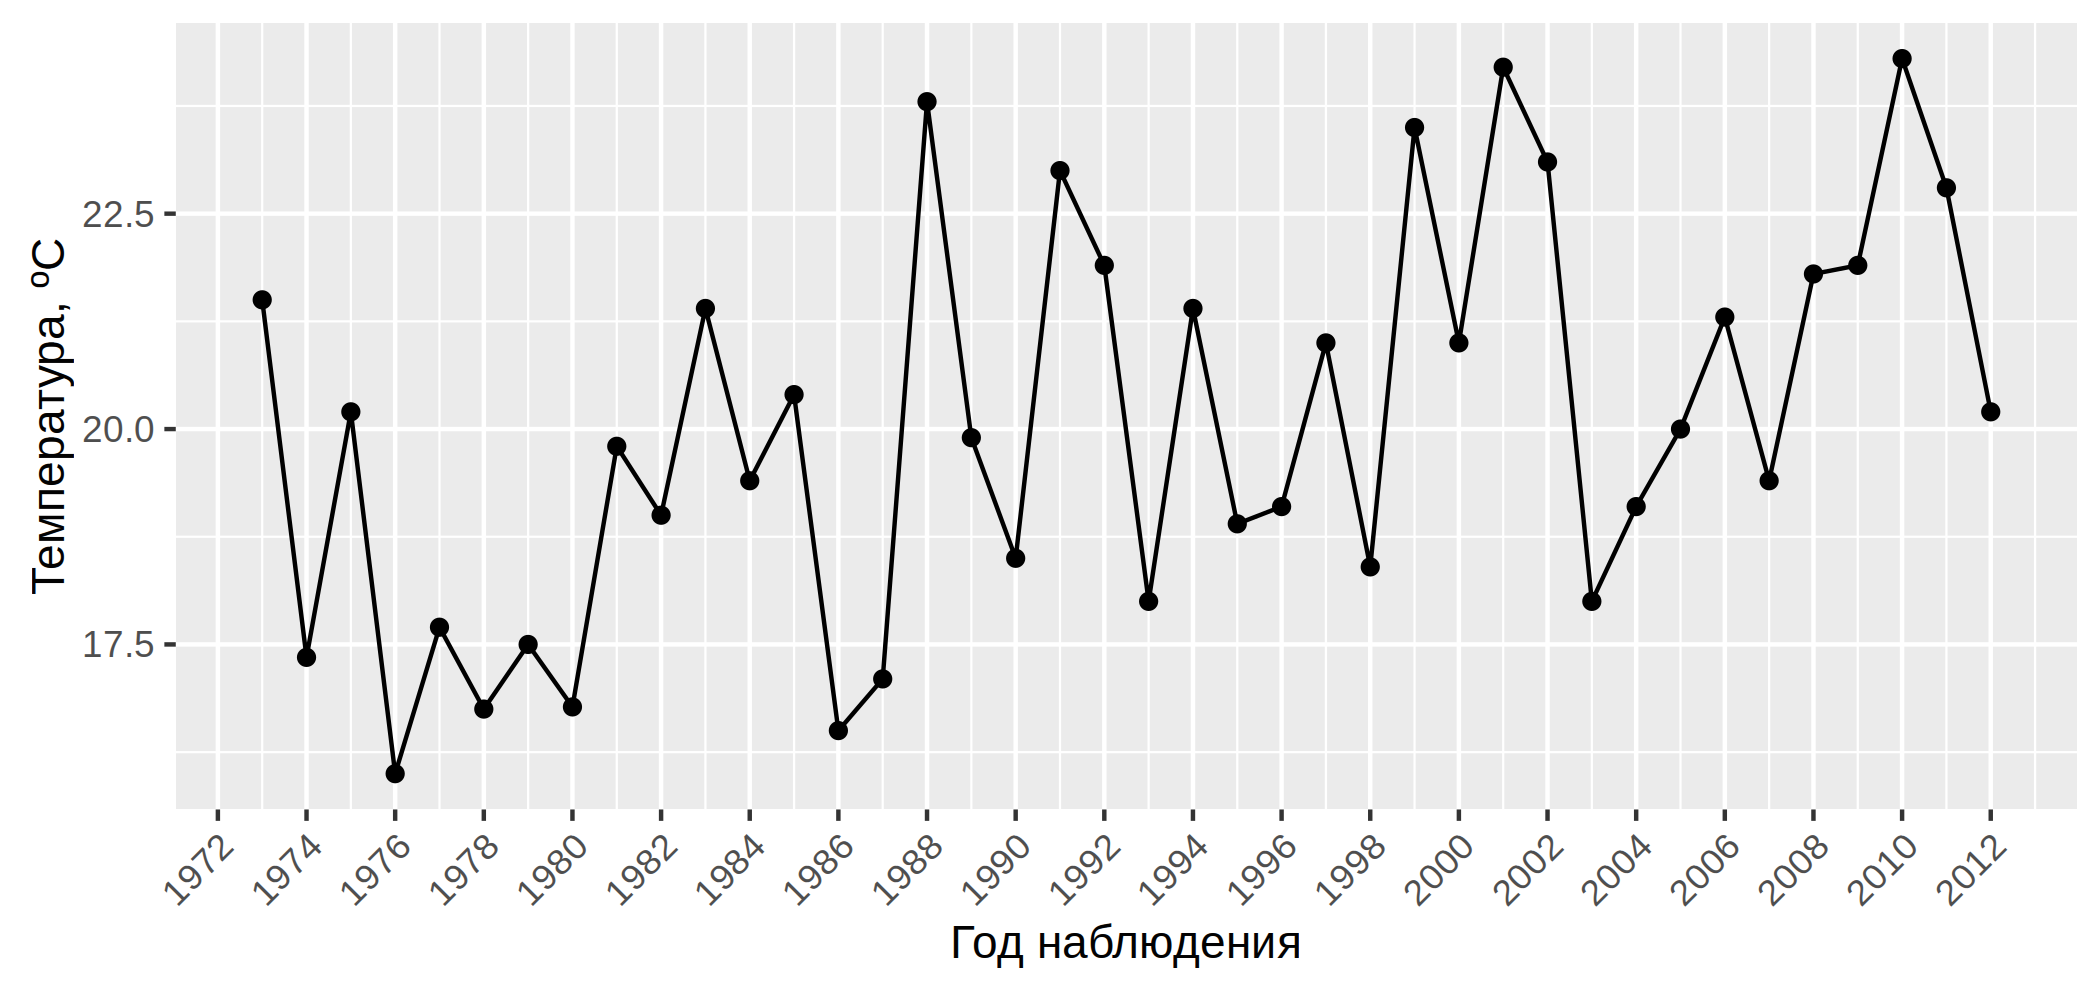
\includegraphics[width=1\linewidth]{../../figures/source.png}
    \caption{Исходные данные}
  \end{figure}
  \end{columns}
  
  \vspace{1em}
  
  Исходные данные представляют собой выборку $ X(t), t = \overline{1,n}, n = 38 $, состоящую из значений средней температуры воды в июле месяце каждый год в период с 1975 по 2012 годы.
\end{frame}

\section{Обзор реализованного ПО}

\begin{frame}
  \frametitle{\large\secname}
  \framesubtitle{Особенности}
  \begin{itemize}
    \item Доступно с любого устройства, имеющего доступ в интернет, по адресу \href{https://apaulau.shinyapps.io/obatorino}{apaulau.shinyapps.io/obatorino};
    \item Реализовано на языке программирования \textbf{R};
    \item Логически разделено на три модуля;
    \item Имеет простой, быстро расширяемый гибкий интерфейс;
    \item Широкие графические возможности;
    \item Проверка тестов и критериев;
    \item Мгновенный отклик на изменение параметров.
  \end{itemize}
\end{frame}

\subsection{Модуль разведочного анализа}

\begin{frame}
  \frametitle{\large\secname}
  \framesubtitle{\subsecname}
    \begin{figure}[h]
    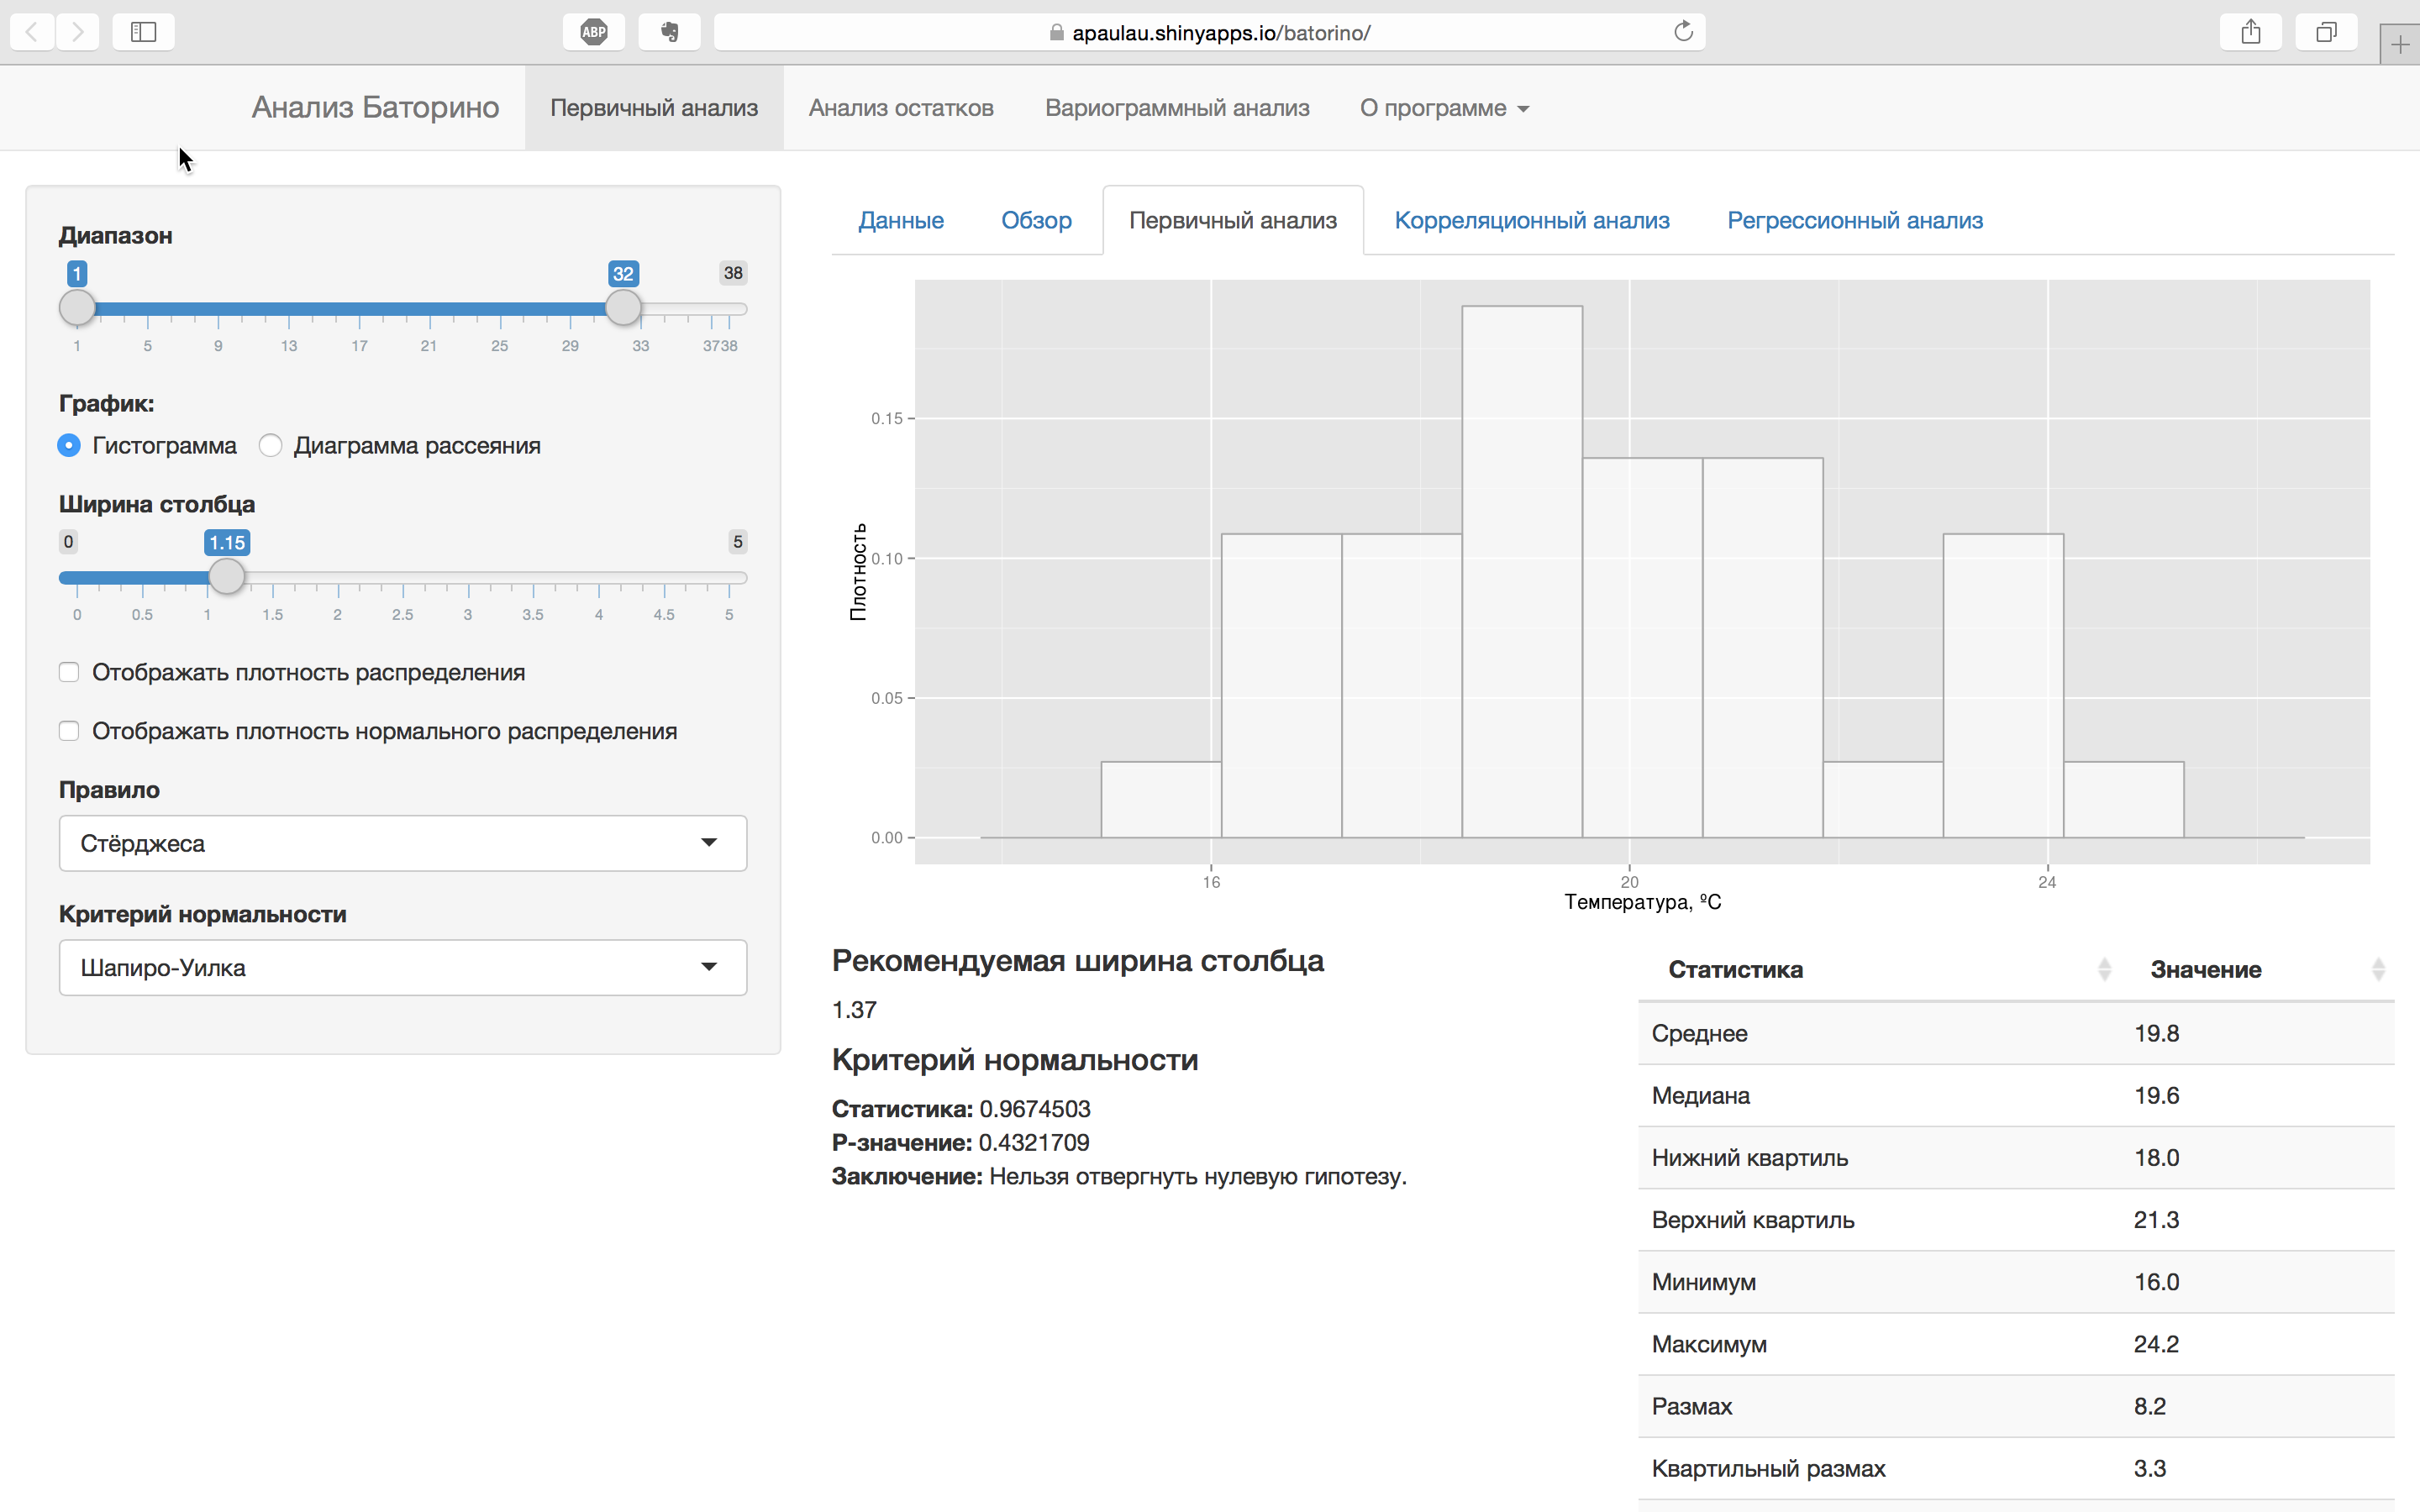
\includegraphics[width=1\textwidth]{../../figures/static/1_basis.png}
    \caption{Первичный анализ и описательные статистики}
  \end{figure}
\end{frame}

\begin{frame}
  \frametitle{Проверка на нормальность}
  \begin{columns}[c]
  \column{0.4\linewidth}
  {\footnotesize
  Выборочное распределение характеризуется небольшой скошенностью вправо (коэффициент асимметрии $ \descriptive{original}{skew} $) и пологостью пика кривой распределения (коэффициент эксцесса $ \descriptive{original}{kurtosis} $) относительно нормального.
  }

  \column{0.6\linewidth}
  \begin{figure}[h]
    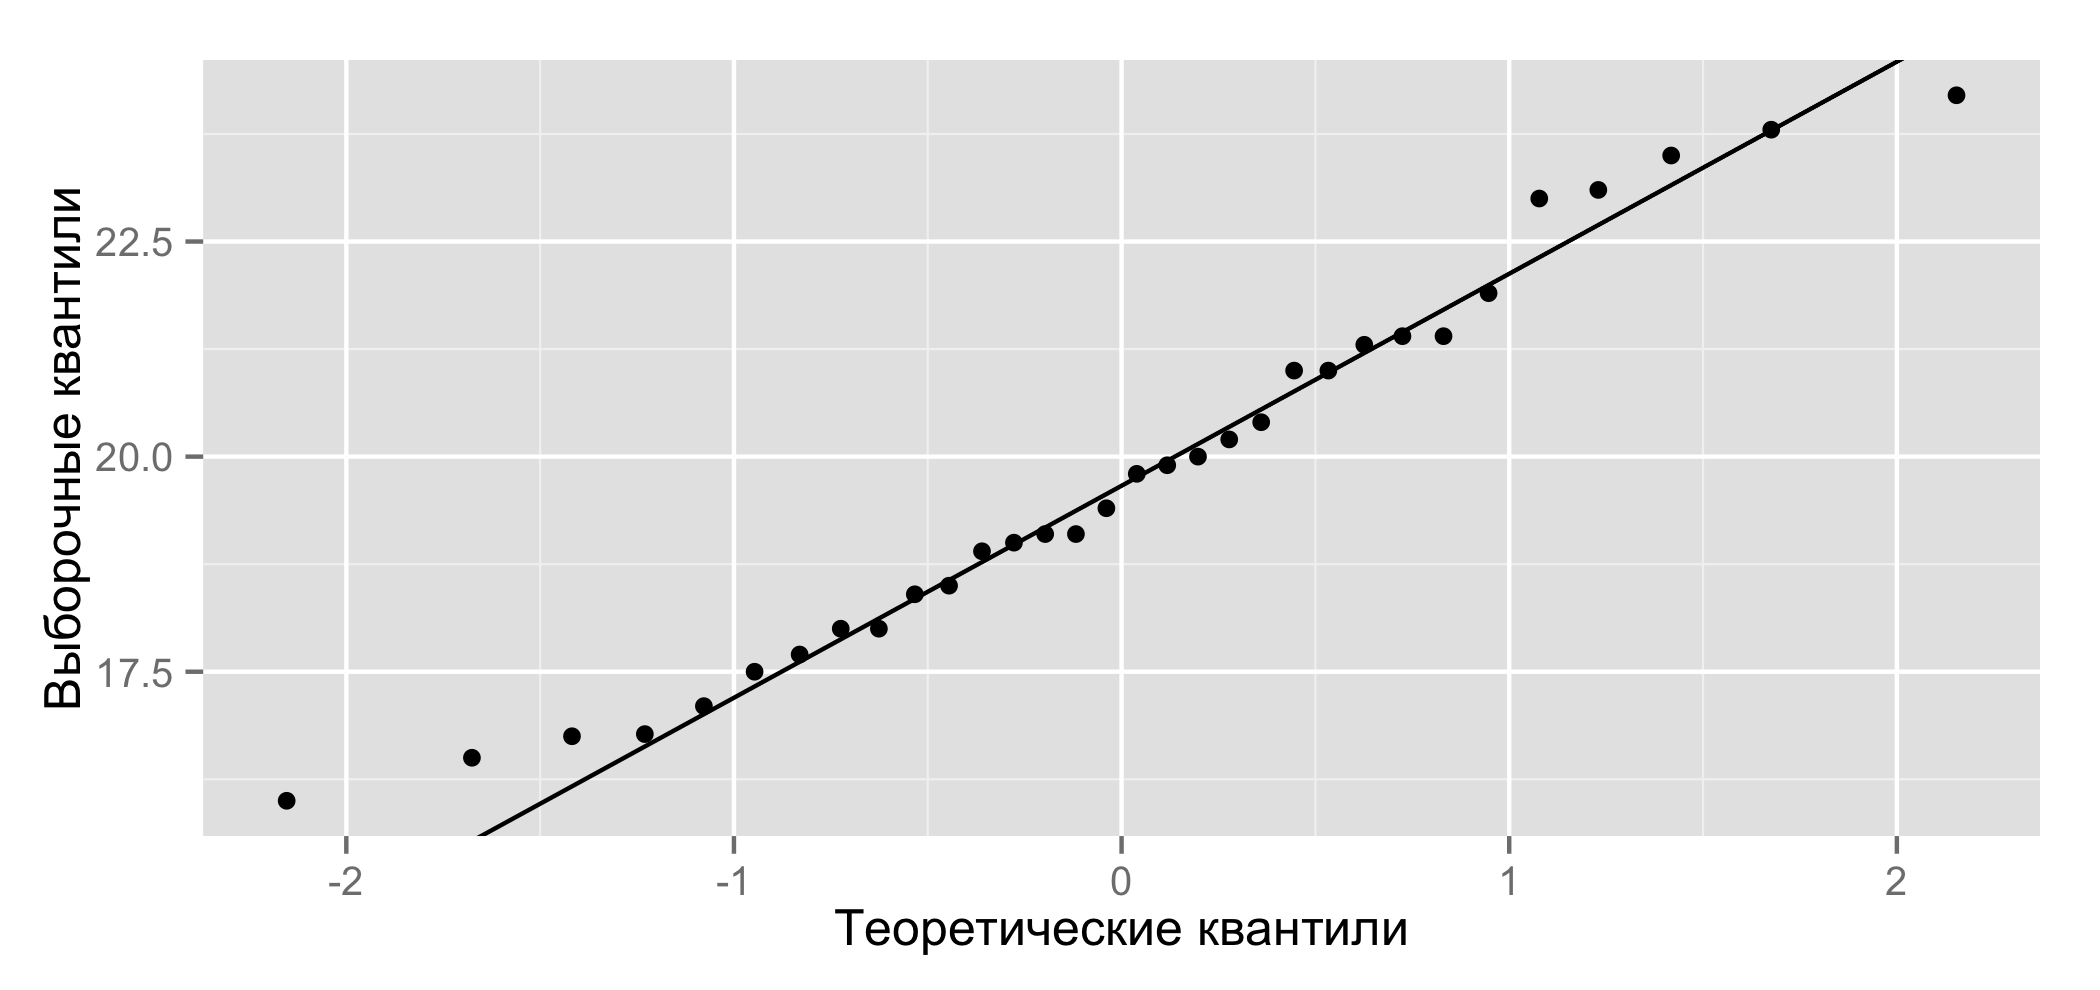
\includegraphics[width=1\linewidth]{../../figures/original/quantile.png}
    \caption{График квантилей}
  \end{figure}
  \end{columns}
  
  \vspace{1em}
  
  Визуально и проверкой критериев Шапиро-Уилка, $\chi^2$-Пирсона и Колмогорова-Смирнова была показана близость выборочного распределения к нормальному с параметрами \normaldistr.
\end{frame}

\begin{frame}
  \frametitle{\large\secname}
  \framesubtitle{\subsecname}
  \begin{figure}[h]
    \center{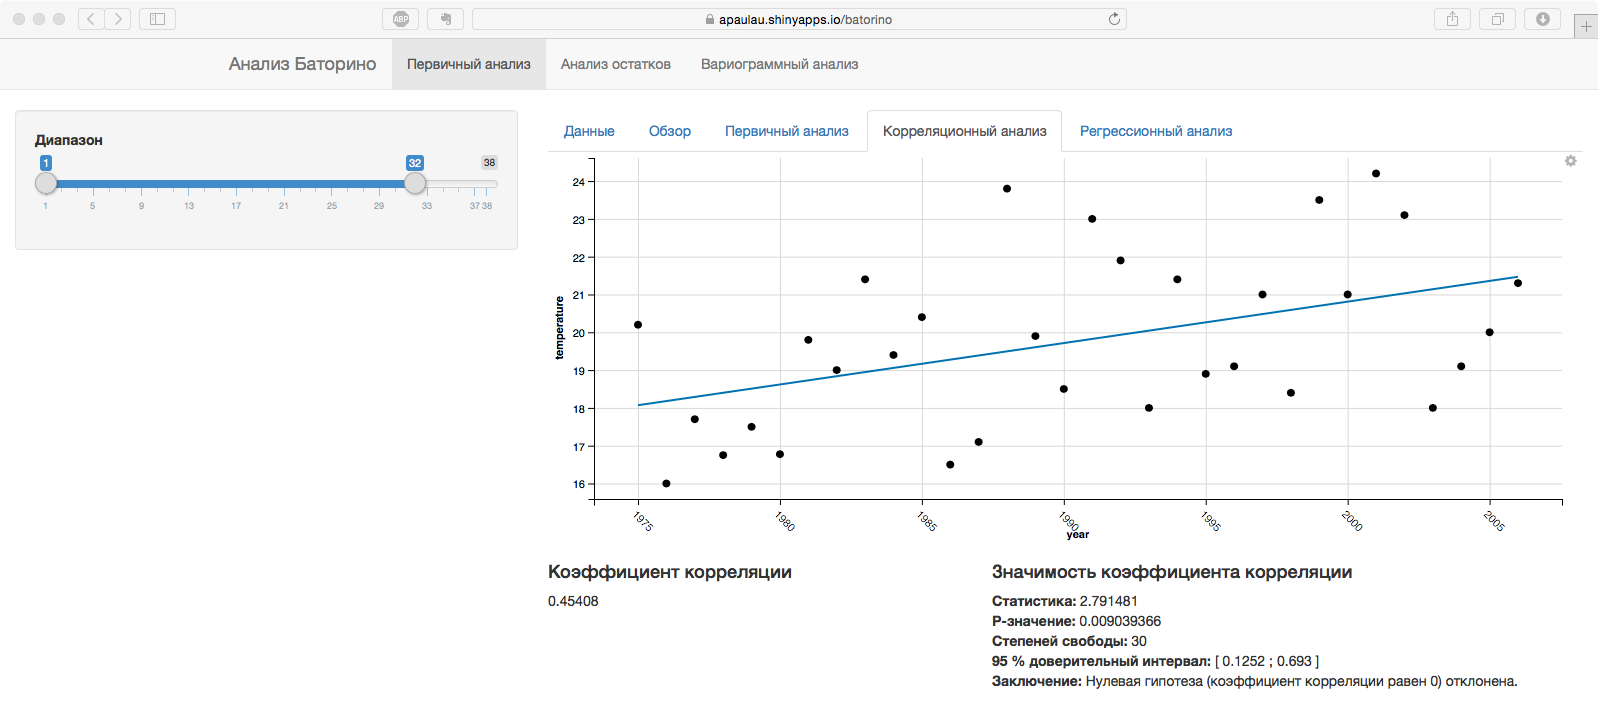
\includegraphics[width=1\textwidth]{../../figures/static/p_corr.png}}
    \caption{Корреляционный анализ}
  \end{figure}
\end{frame}

\begin{frame}
  \frametitle{\large\secname}
  \framesubtitle{\subsecname}
    \begin{figure}[h]
    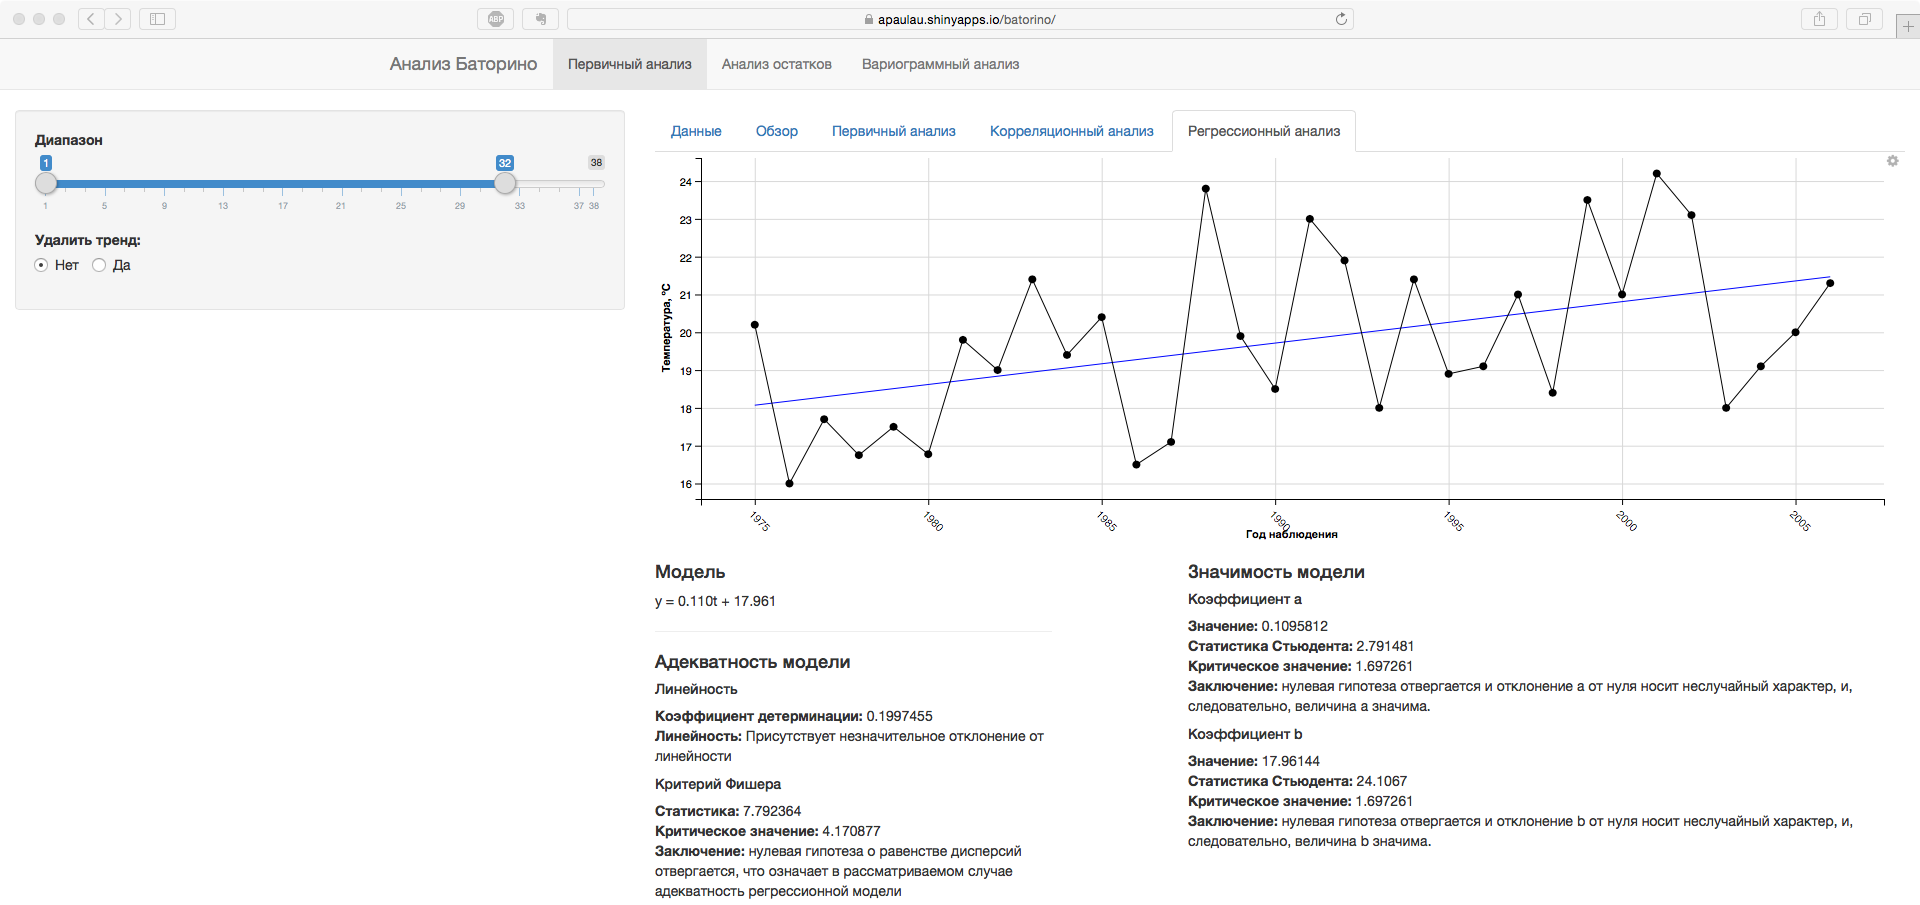
\includegraphics[width=1\textwidth]{../../figures/static/2_regr.png}
    \caption{Регрессионный анализ}
  \end{figure}
\end{frame}

\begin{frame}
  \frametitle{Регрессионная модель}
  Модель исследуемого временного ряда является аддитивной:
  \begin{equation}
    X(t) = y(t) + \varepsilon(t),
  \end{equation}
  где $ y(t) $ --- тренд, $ \varepsilon(t) $ --- нерегулярная составляющая.

  \vspace{0.2em}

  \begin{center}
    Найдена модель тренда: $ y(t) = at + b = 0.1014t + 18.0521 $
  \end{center}
  \begin{columns}[c]
  \column{0.5\linewidth}
  {\footnotesize
  \begin{itemize}
    \item F-критерий Фишера при уровне значимости $ \alpha = 0.05 $ показал адекватность модели
    \item При $ \alpha=0.05 $, с помощью критерия Стьюдента, доказана значимость коэффициентов регрессионной модели
    \item Точность модели невысока, поскольку коэффициент детерминации $ \eta^2_{x(t)} = 0.275 $
  \end{itemize}
  }
  \column{0.5\linewidth}
  {\footnotesize
  % latex table generated in R 3.1.3 by xtable 1.7-4 package
% Thu May 21 14:09:02 2015
\begin{table}[ht]
\centering
\begin{tabular}{rrrr}
  \hline
 & Год & Актуальное & Прогнозное \\ 
  \hline
1 & 2007 & 19.40 & 18.07 \\ 
  2 & 2008 & 21.80 & 18.18 \\ 
  3 & 2009 & 21.90 & 18.29 \\ 
  4 & 2010 & 24.30 & 18.40 \\ 
  5 & 2011 & 22.80 & 18.51 \\ 
  6 & 2012 & 20.20 & 18.62 \\ 
   \hline
\end{tabular}
\caption{Сравнение прогнозных значений (тренда)} 
\label{table:prediction_trend}
\end{table}

  }
  \end{columns}
\end{frame}

\subsection{Модуль анализа остатков}

\begin{frame}
  \frametitle{\large\secname}
  \framesubtitle{\subsecname}
    \begin{figure}[h]
    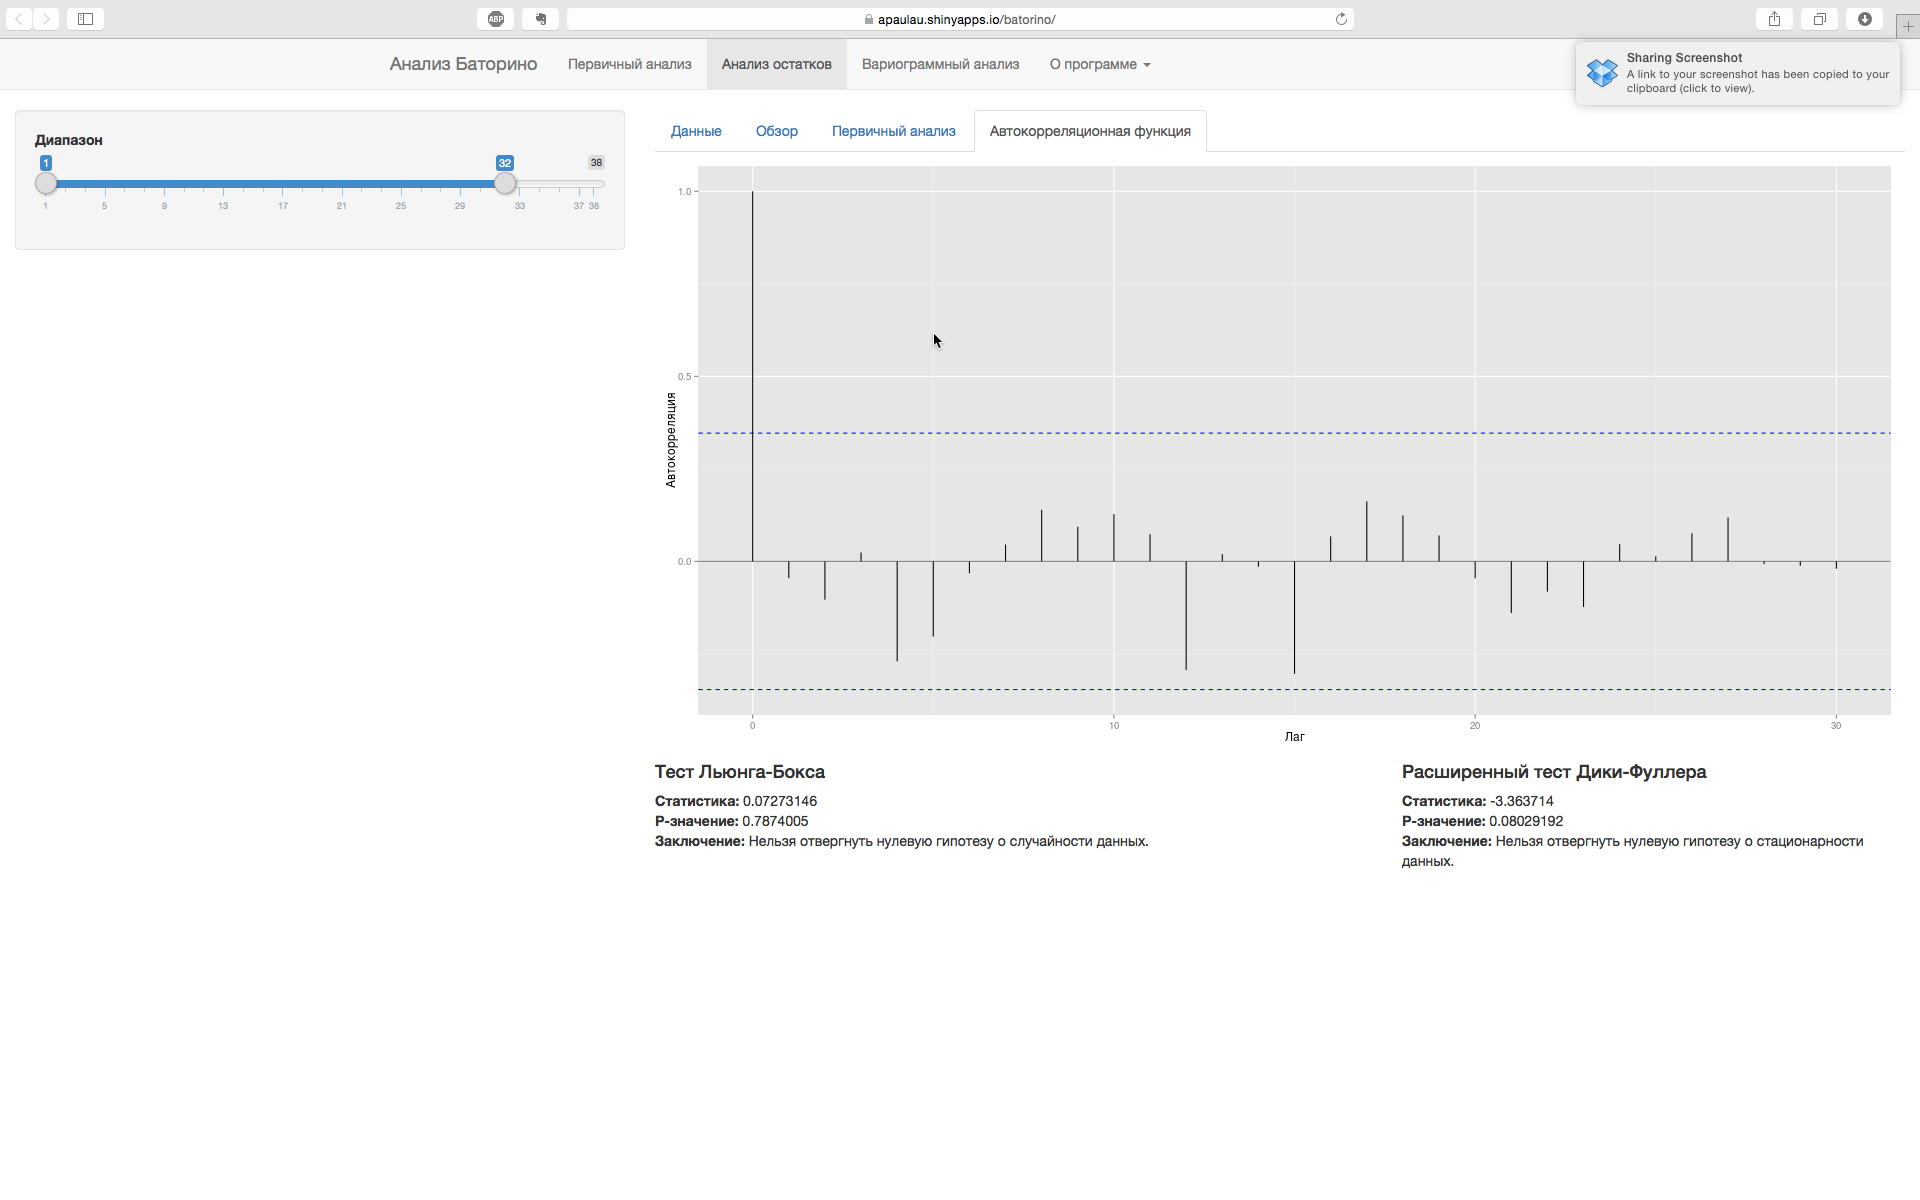
\includegraphics[width=1\textwidth]{../../figures/static/3_acf.png}
    \caption{Автокорреляционная функция}
  \end{figure}
\end{frame}

\begin{frame}
  \frametitle{Анализ остатков}
  \begin{itemize}
    \item Визуально и проверкой тестов показана близость выборочного распределения к нормальному \resnormaldistr;
    \item По графику и тестом Льюнга-Бокса сделано заключение об отсутствии значимых автокорреляций;
    \item Значения имеют небольшую амплитуду и имеют тенденцию к затуханию. Это говорит о стационарности в широком смысле, что показал расширенный тест Дики-Фуллера.
  \end{itemize}
\end{frame}

\subsection{Модуль вариограммного анализа}

\begin{frame}
\begin{footnotesize}
  \frametitle{Оценка вариограммы}
  \begin{Definition}
    \textit{Вариограммой} случайного процесса $ X(t), t \in \mathbb{Z} $, называется функция вида
    \begin{equation}
    \label{eq:matheron}
        2 \gamma (h) = V \{ X(t + h) - X(t) \},~ t, h \in \mathbb{Z}.
    \end{equation}

    При этом функция $ \gamma (h), h \in \mathbb{Z} $, $ \gamma(h) = \gamma(-h)$, называется \textit{семивариограммой}.
  \end{Definition}
  
  \vspace{0.5em}
  
  Рассматривается стационарный в широком смысле гауссовский случайный процесс с дискретным временем $ X(t),~ t \in \mathbb{Z} $, нулевым математическим ожиданием, постоянной дисперсией и неизвестной вариограммой $ 2 \gamma(h), h \in \mathbb{Z} $.
\end{footnotesize}
  
  \vspace{0.5em}
  
  В качестве оценки вариограммы рассматривается статистика, предложенная Матероном:
  \begin{equation}
    2 \tilde{\gamma}(h) = \frac{1}{n - h} \sum_{t = 1}^{n - h}(X(t + h) - X(t))^2, \quad h = \overline{0, n - 1},
  \end{equation}

  \vspace{-0.4em}
  \begin{footnotesize}
  где $ \tilde{\gamma}(-h) = \tilde{\gamma}(h), h = \overline{0, n - 1}; \tilde{\gamma}(h) = 0, |h| \ge n $.
  \end{footnotesize}
\end{frame}

\begin{frame}
  \frametitle{Вариограммный анализ}
  \begin{columns}[c]
  \column{0.5\linewidth}
    Прогнозные значения $ X^{*}(t) $ вычисляются по формуле:
    \begin{equation*}
      X^{*}(t) = y(t) + \varepsilon^{*}(t),
    \end{equation*}
    где $ y(t) $ --- тренд, $ \varepsilon^{*}(t) $ --- значения, вычисленные с помощью кригинга.

  \column{0.5\linewidth}
    \begin{figure}[h]
    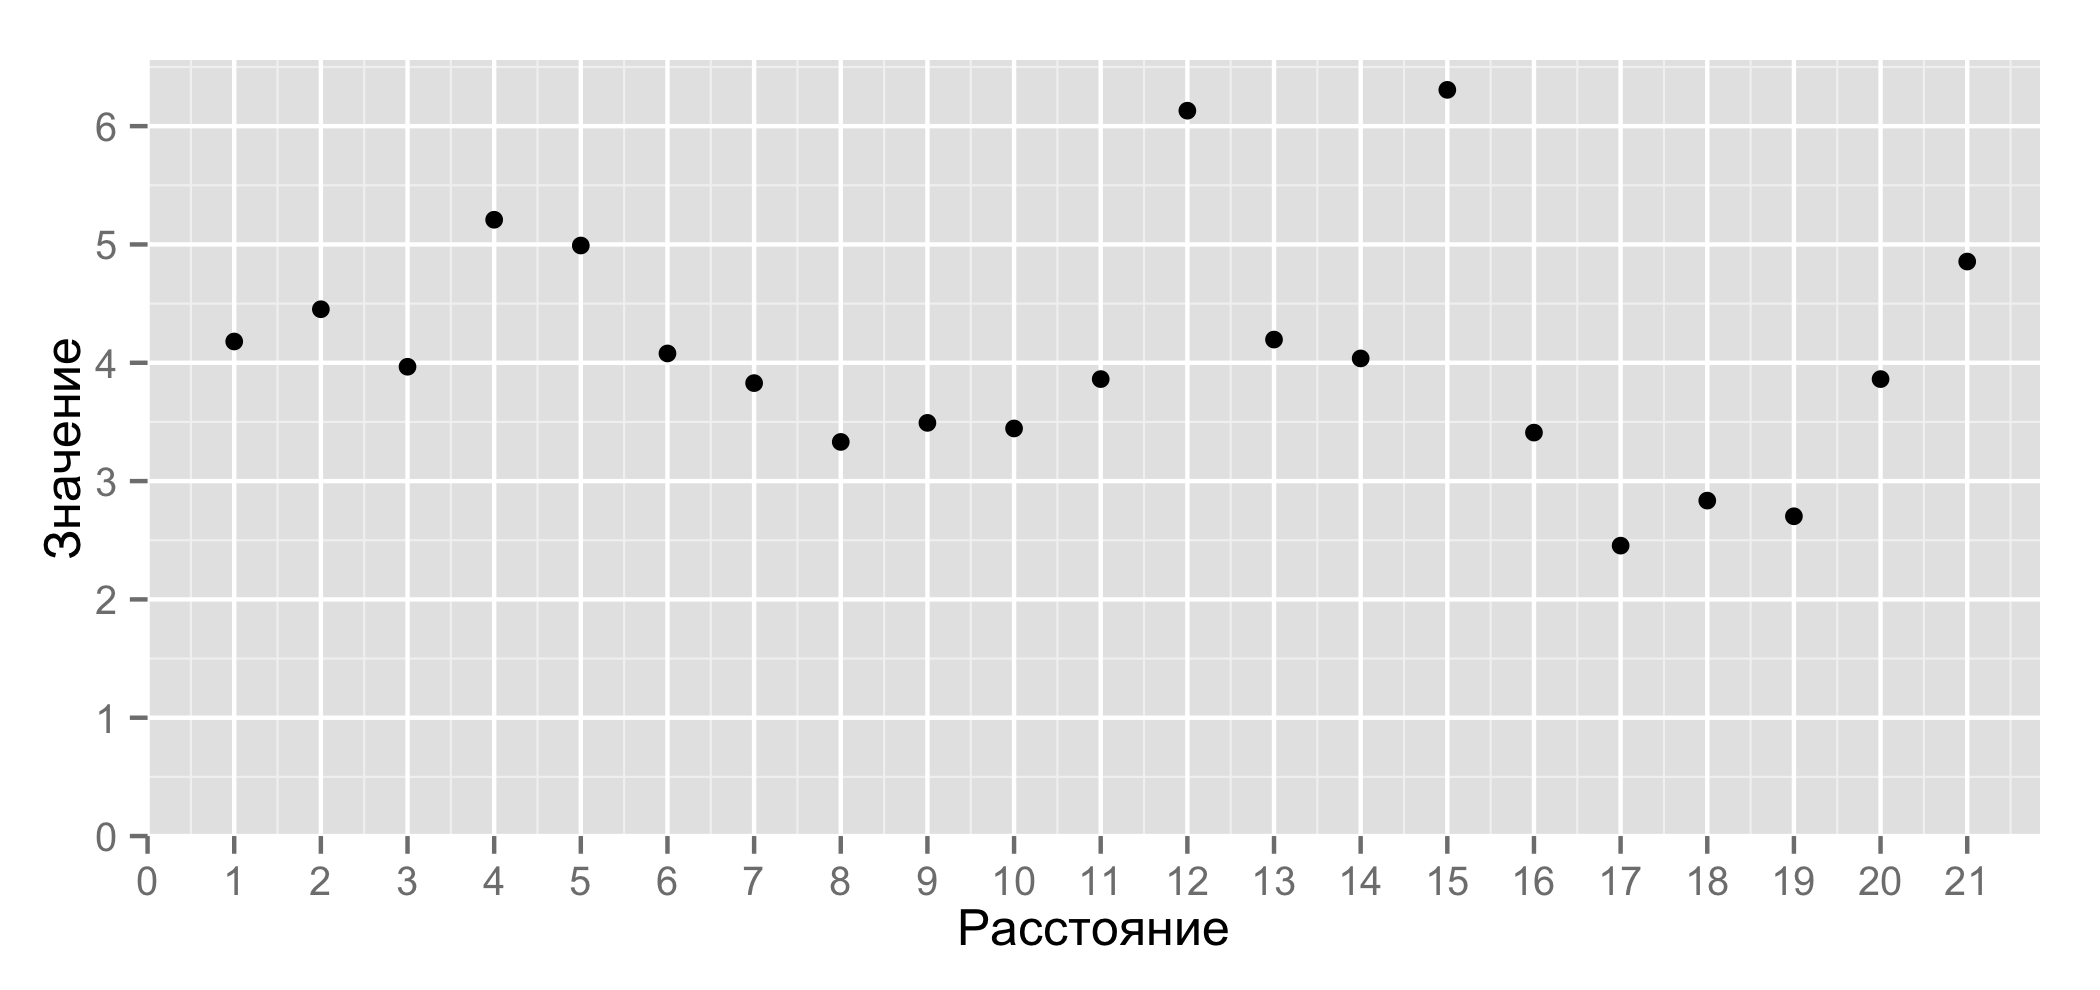
\includegraphics[width=1\linewidth]{../../figures/variogram/lin-variogram.png}
    \caption{Оценка семивариограммы Матерона}
  \end{figure}
  \end{columns}
  
  \vspace{1em}
  
  Для оценки качества модели используются
  \begin{itemize}
    \item коэффициент корреляции $ r_{\varepsilon\varepsilon^{*}} $
    \item Среднеквадратическая ошибка
    \begin{equation}
      \label{eq:mse}
      MSE = \frac{1}{n} \sum_{i=1}^{n} (\varepsilon(t_i) - \varepsilon^{*}(t_i))^2,
    \end{equation}
    где $ n $ --- объём выборки
  \end{itemize}
\end{frame}

\begin{frame}
  \frametitle{\large\secname}
  \framesubtitle{\subsecname}
    \begin{figure}[h]
    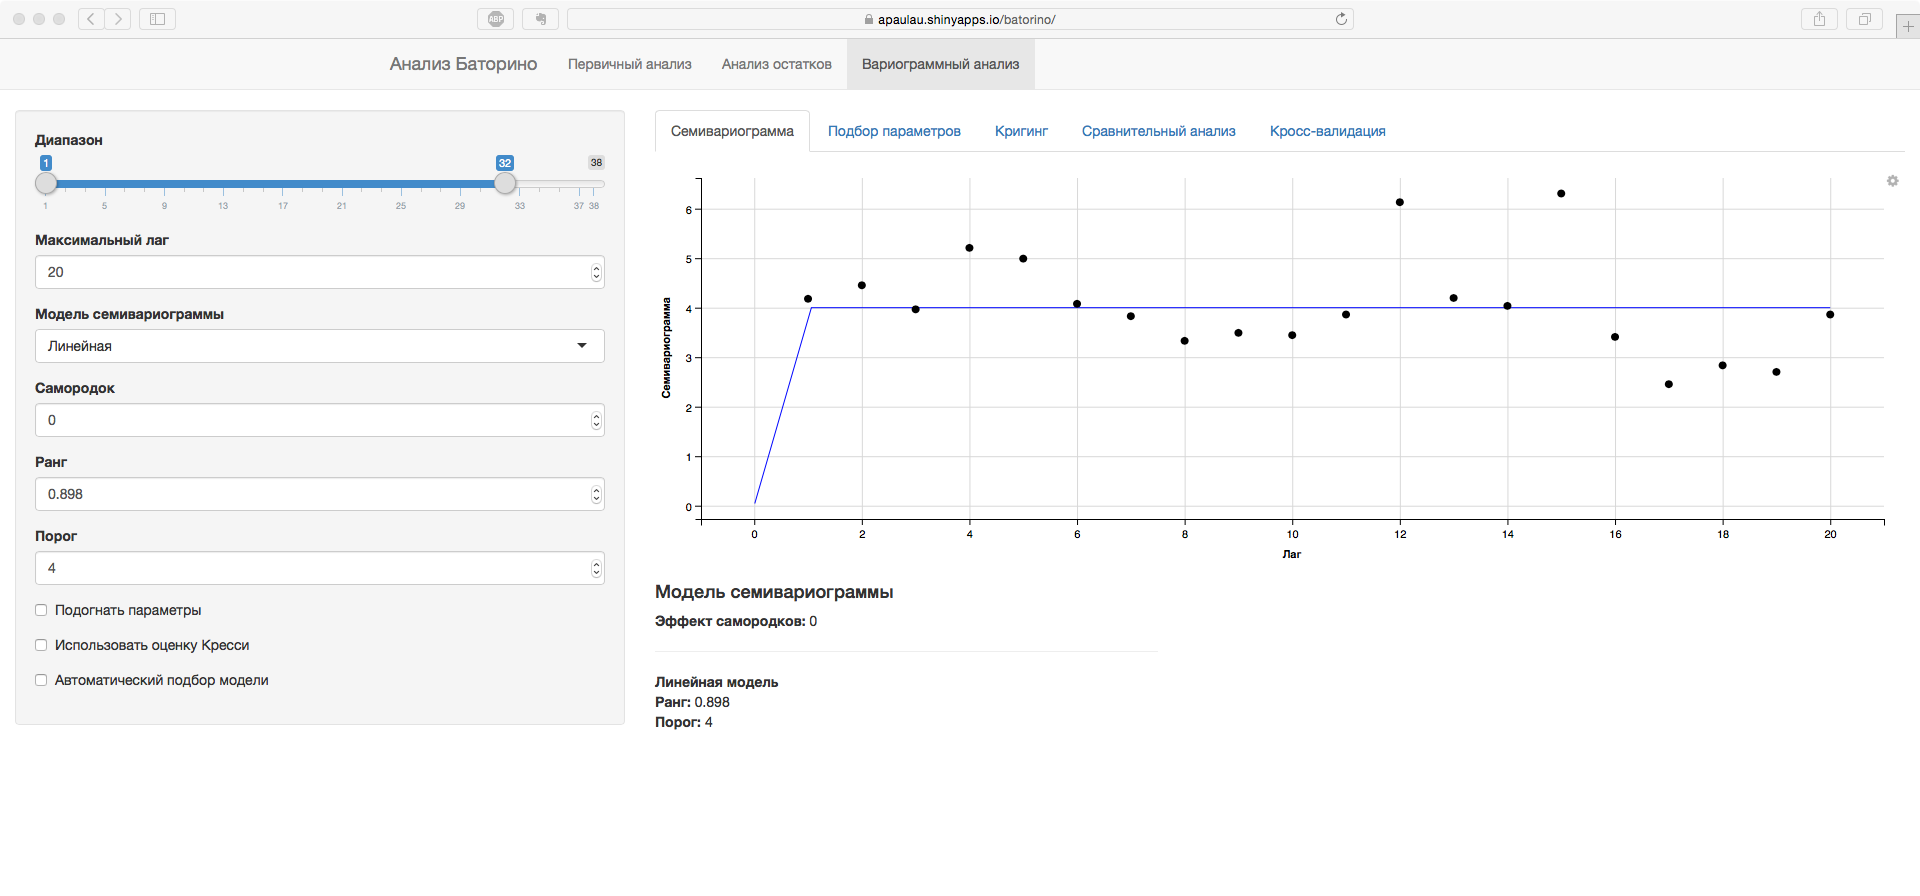
\includegraphics[width=1\textwidth]{../../figures/static/4_variogram.png}
    \caption{Возможности по подбору модели семивариограммы}
  \end{figure}
\end{frame}

\begin{frame}
  \frametitle{\large\secname}
  \framesubtitle{\subsecname}
    \begin{figure}[h]
    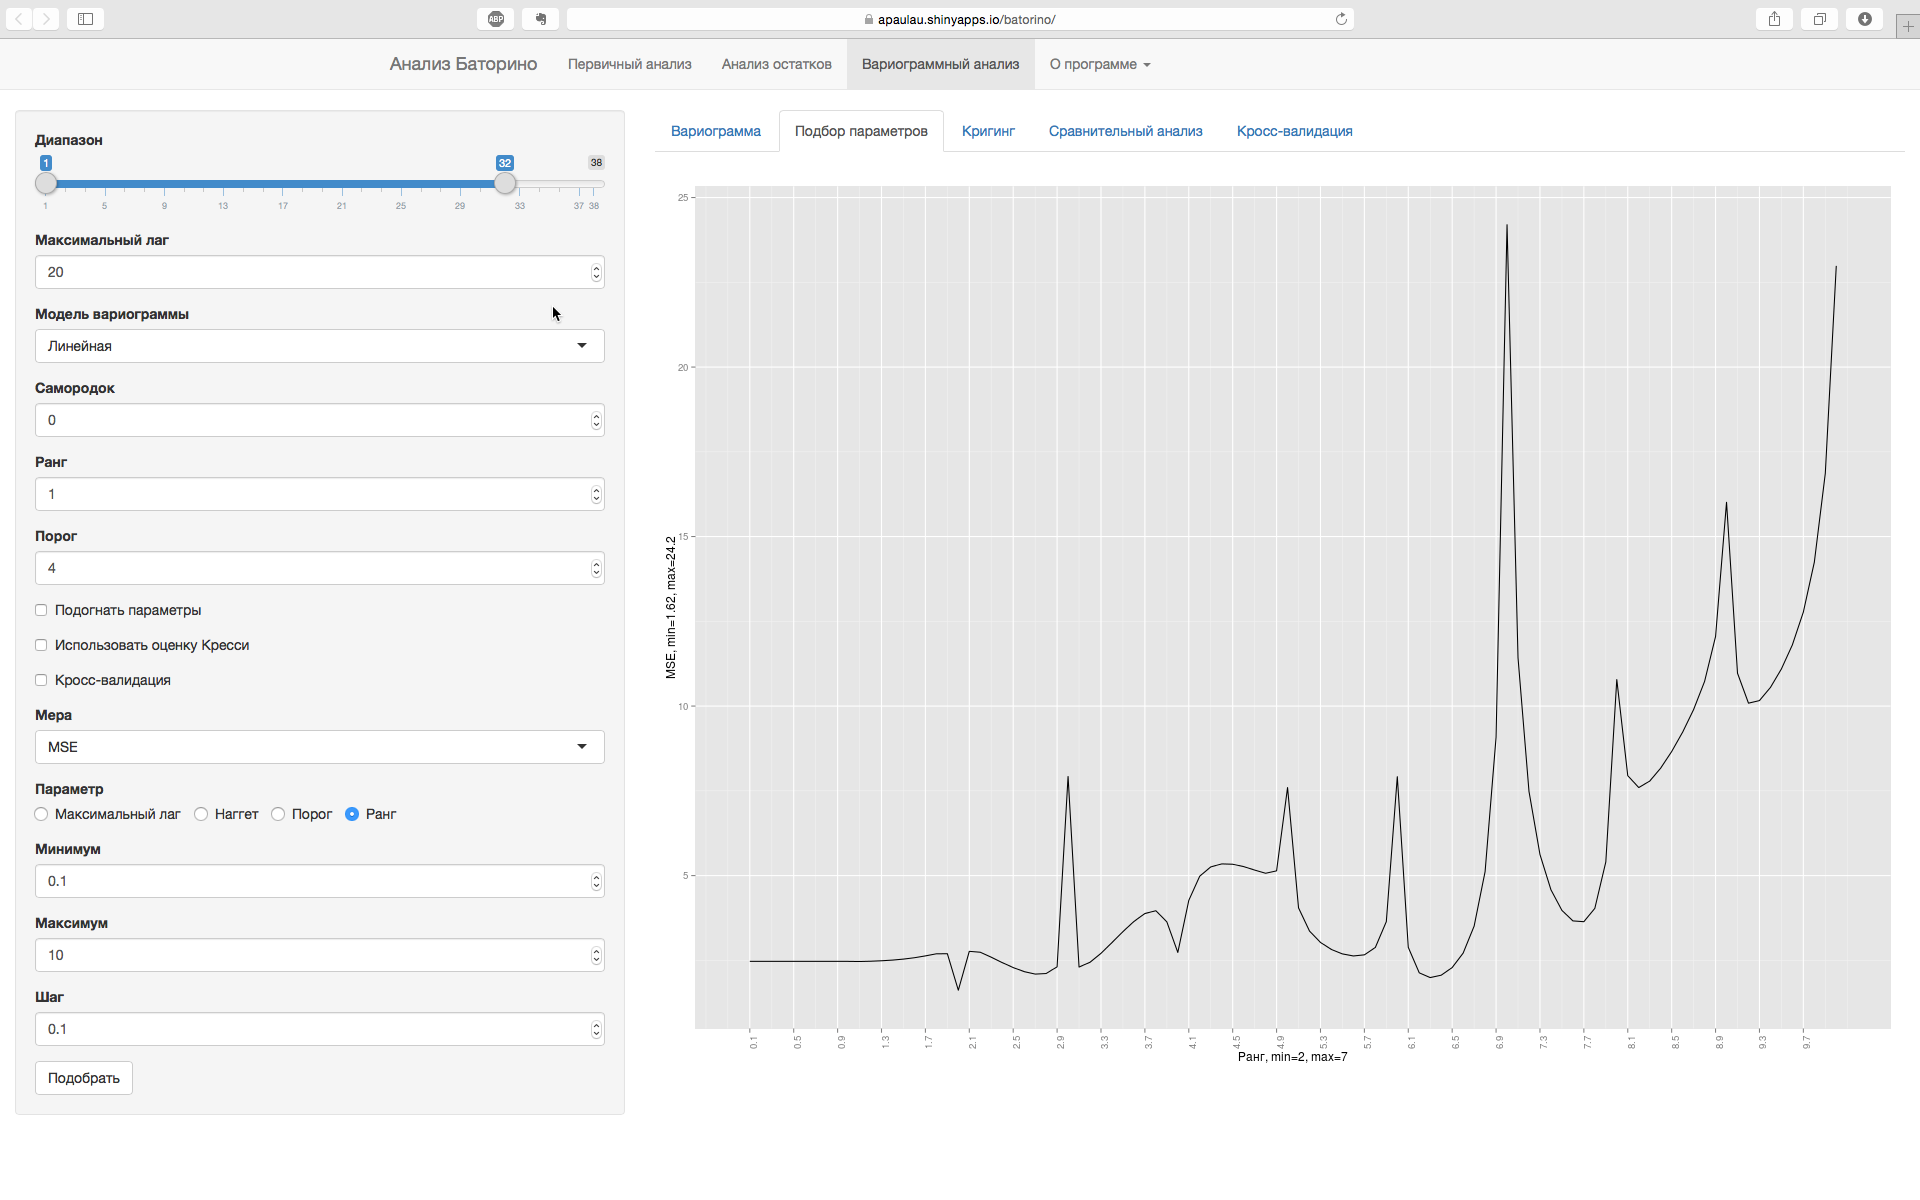
\includegraphics[width=1\textwidth]{../../figures/static/5_fit.png}
    \caption{Подбор параметров модели семивариограммы}
  \end{figure}
\end{frame}

\begin{frame}
  \frametitle{\large\secname}
  \framesubtitle{\subsecname}
    \begin{figure}[h]
    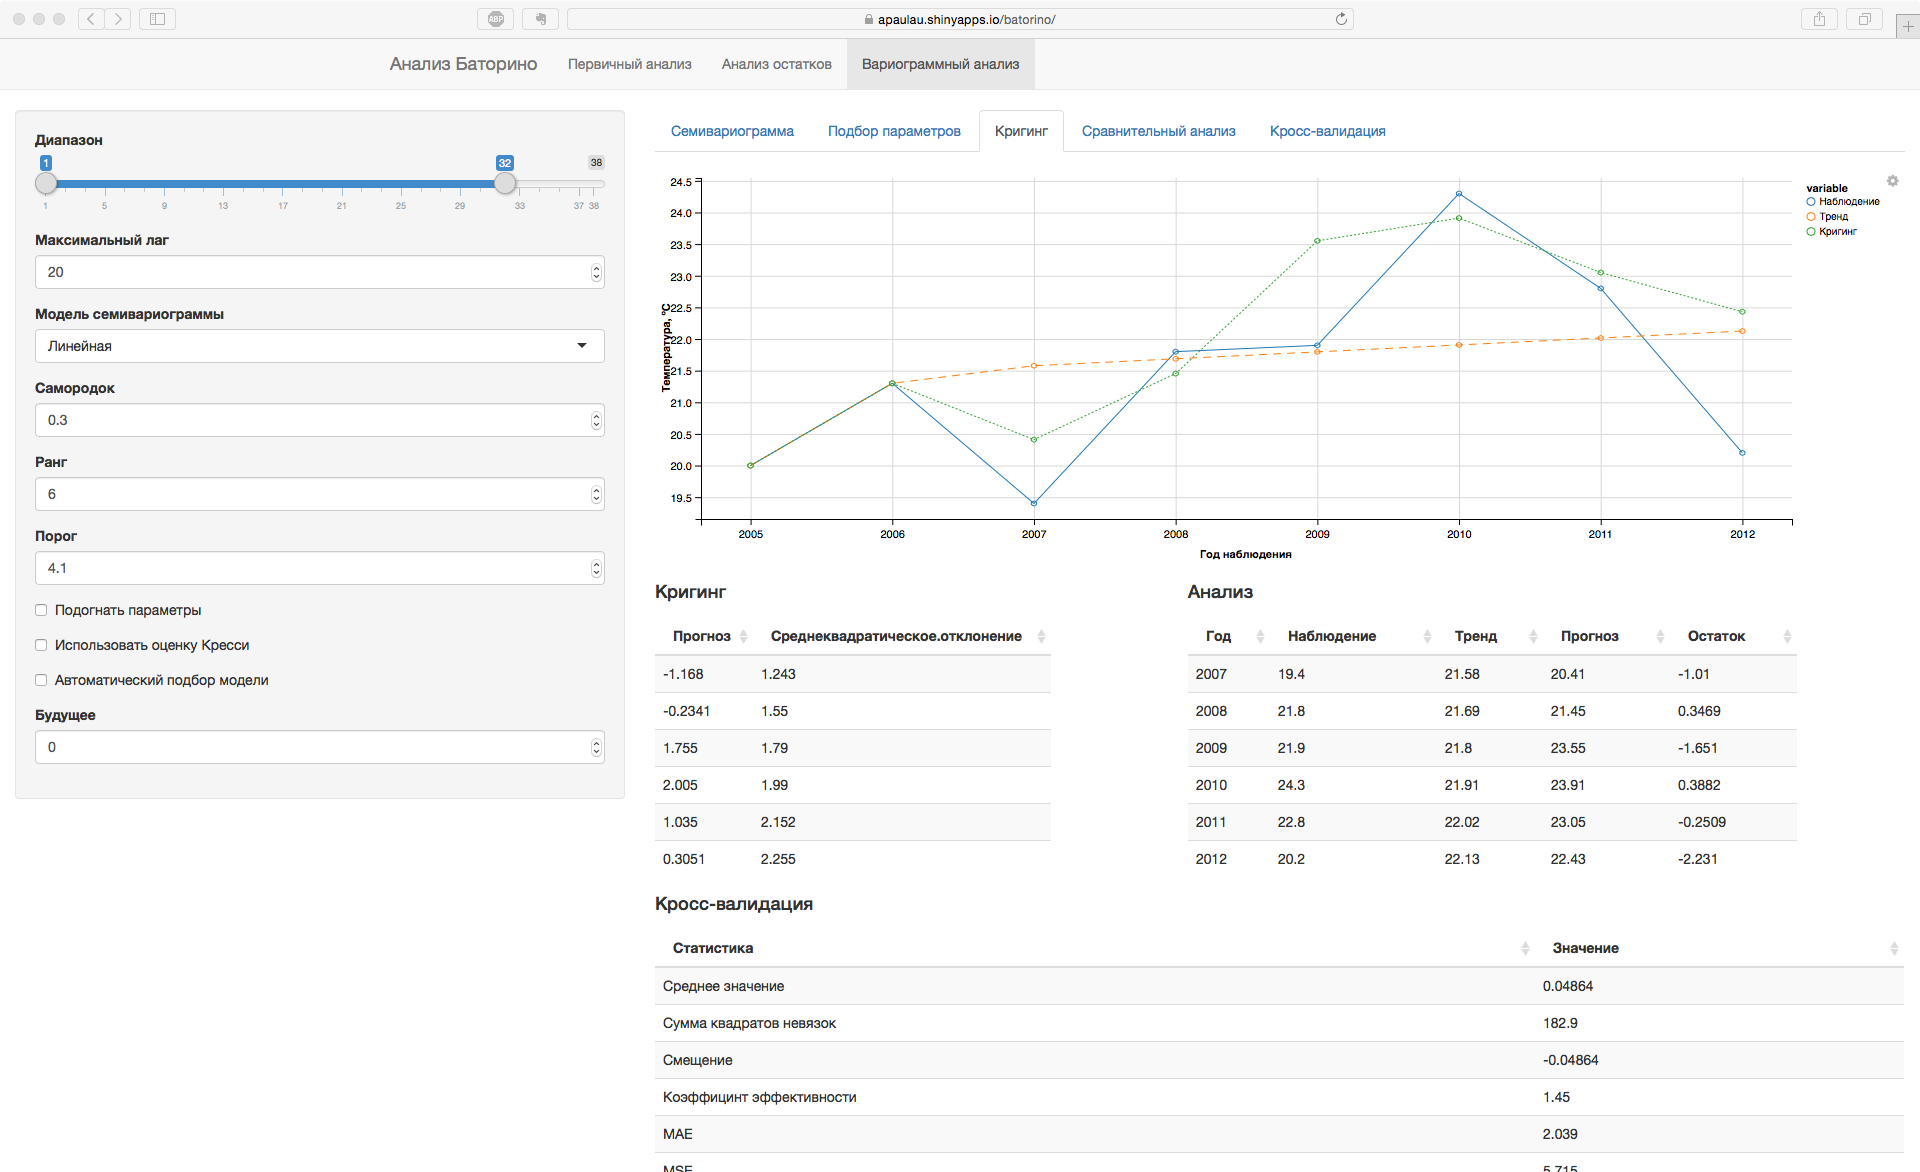
\includegraphics[width=1\textwidth]{../../figures/static/6_krige.png}
    \caption{Сравнение прогнозных значений}
  \end{figure}
\end{frame}

\subsection{Визуальный подход}%Вариограммный анализ}

\begin{frame}
  \frametitle{\large\subsecname}
  \framesubtitle{Линейная модель}
  \begin{columns}[c]
  \column{0.42\linewidth}
  {\footnotesize
  \begin{equation}\begin{gathered}
  \label{eq:lin}
    \widehat{\gamma}(h) = c_0 + Lin(h) = \\
    = \left\{
   \begin{array}{l l}
     c_0 + b \cdot h, & h > 0, \\
     c_0, & h = 0,
   \end{array} \right.
  \end{gathered}\end{equation}
  где $ b $ -- параметр, отвечающий за угол наклона, $ c_0 $ --- эффект самородков.

  \vspace{0.5em}

  Подобранная модель:
  \begin{equation}
  \label{eq:gamma1}
    \widehat{\gamma}_1(h) = Lin(h), \quad b = 4,
  \end{equation}

  Показатели качества
  \begin{equation*}
    r_{\varepsilon\varepsilon^{*}} = -0.09129, \quad MSE = 6.324
  \end{equation*}
  }

  \column{0.58\linewidth}
  \vspace{-14.5pt}
  \begin{figure}[H]
    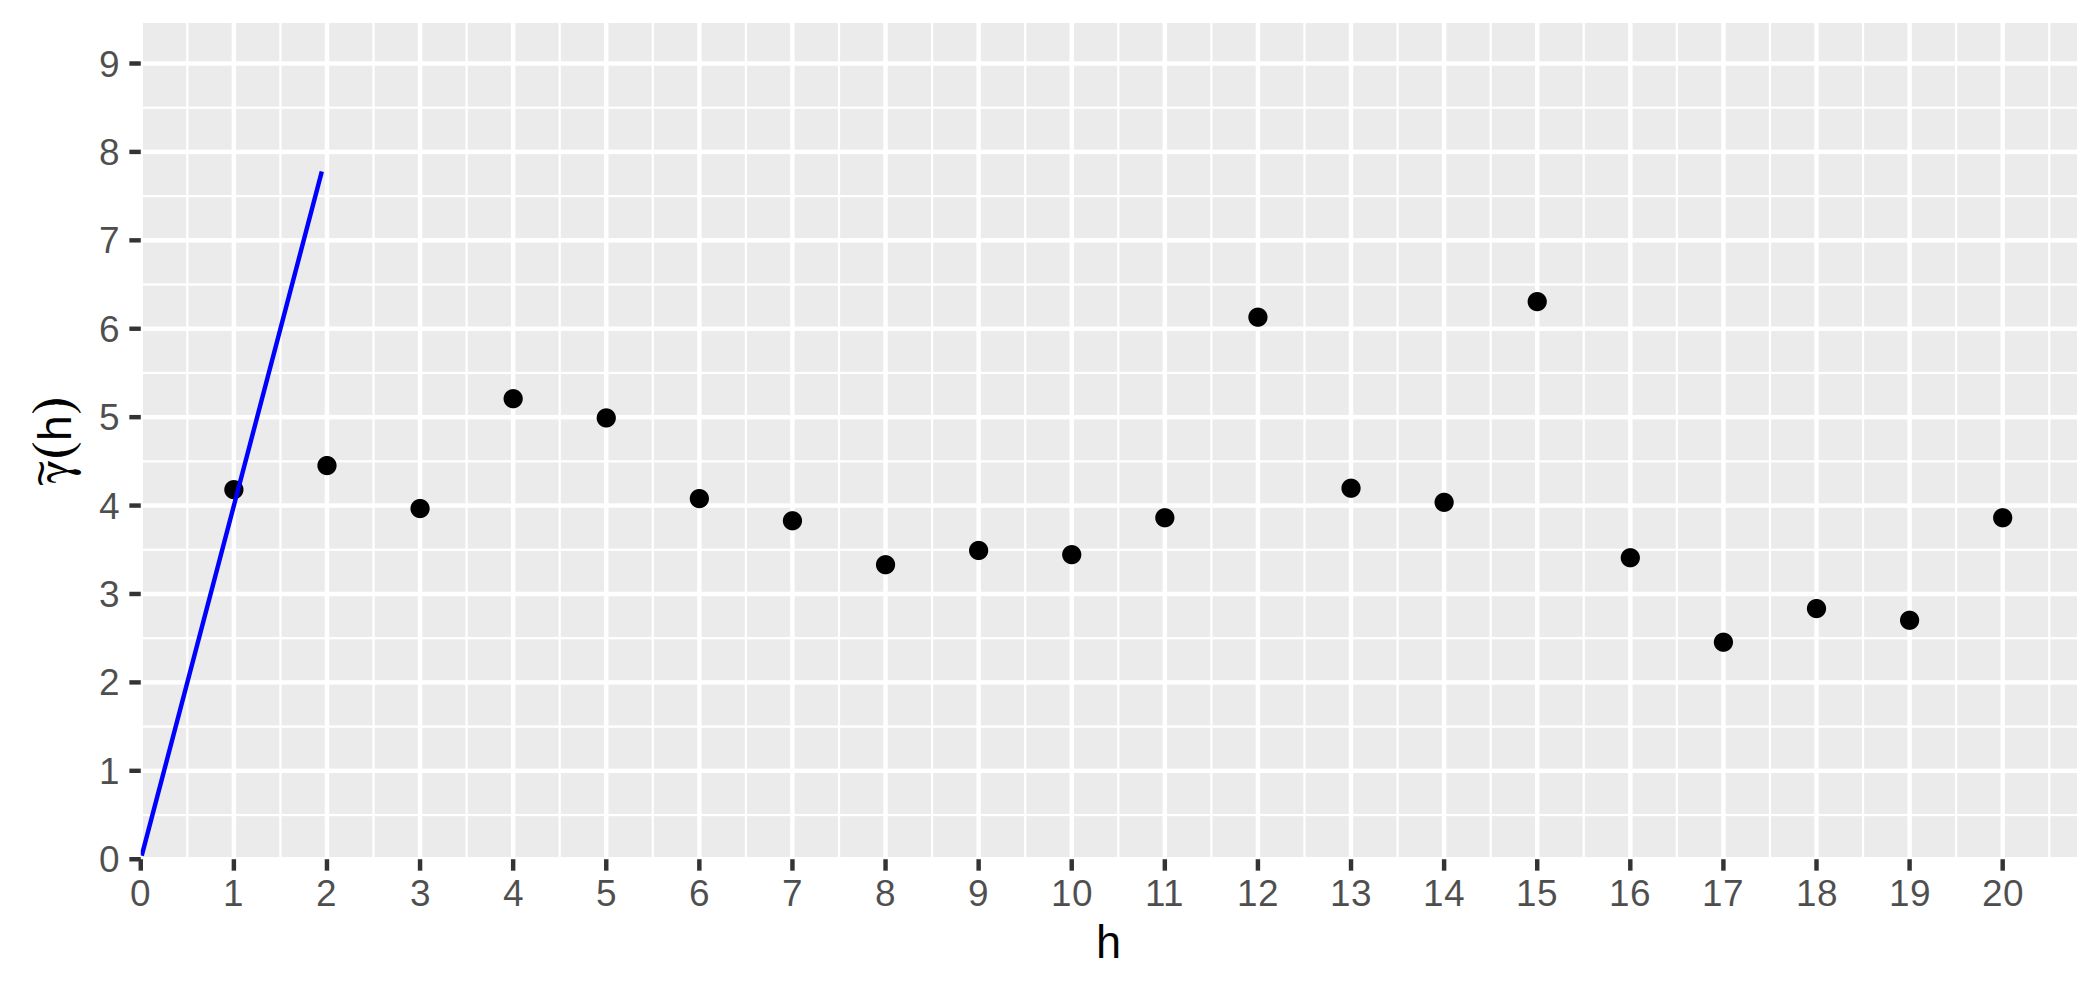
\includegraphics[width=0.9\linewidth]{../../figures/variogram/lin-modeled.png} \\
    \caption{Модель семивариограммы $\widehat{\gamma}_1(h)$}
    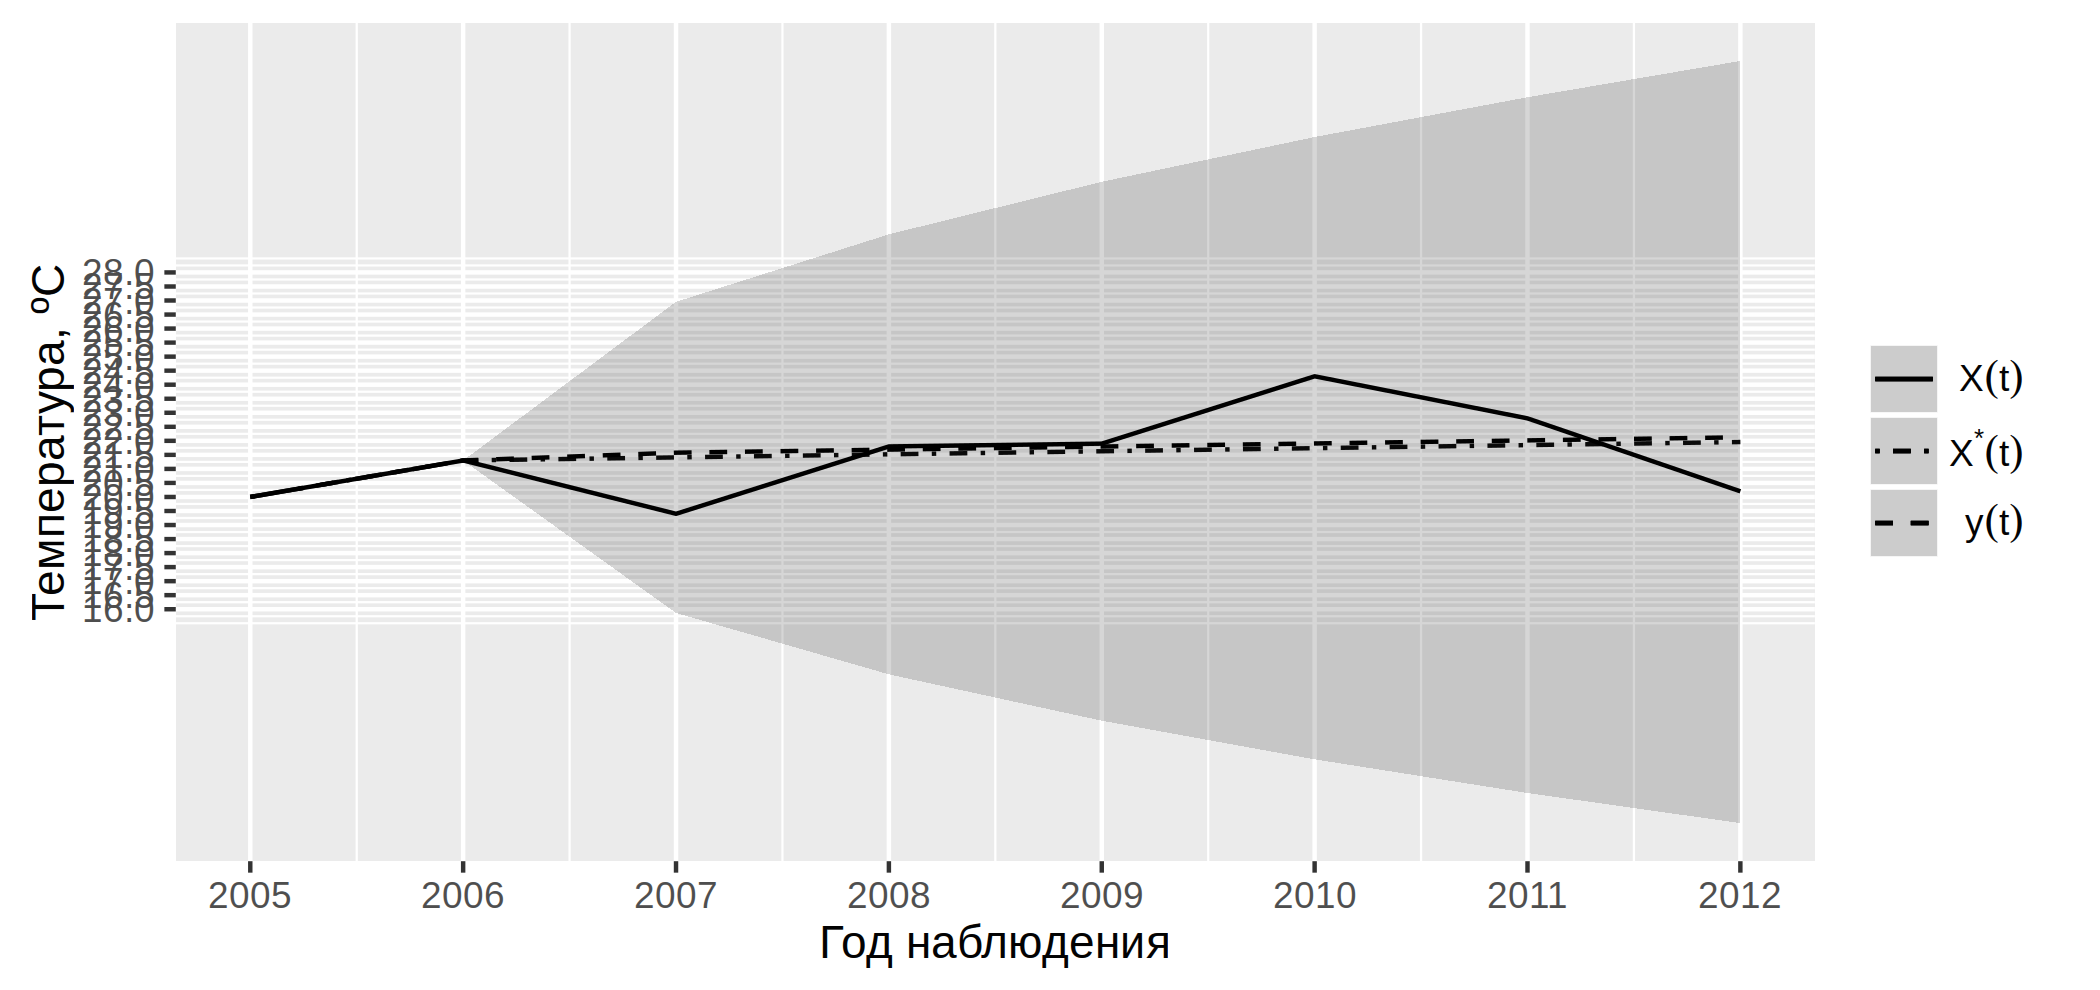
\includegraphics[width=0.9\linewidth]{../../figures/variogram/lin-cross-prediction.png}
    \caption{Прогноз по модели $\widehat{\gamma}_1(h)$}
  \end{figure}
  \end{columns}
\end{frame}

% \begin{frame}
%   \frametitle{\large\subsecname}
%   \framesubtitle{Чистый эффект самородков}
%   \begin{columns}[c]
%   \column{3in}
%   \begin{equation}\begin{gathered}
%   \label{eq:nug}
%     \widehat{\gamma}(h) = c \cdot Nug(h) = \left\{
%    \begin{array}{l l}
%      0, & h = 0, \\
%      c, & h \neq 0.
%    \end{array} \right.
%   \end{gathered}\end{equation}

%   \vspace{0.5em}

%   Подобранная модель:
%   \begin{equation}
%   \label{eq:gamma2}
%     \widehat{\gamma}_2(h) = 4.04 \cdot Nug(h).
%   \end{equation}

%   Показатели качества
%   \begin{equation*}
%     r_{\varepsilon\varepsilon^{*}} = -0.04, \quad MSE = 4.199
%   \end{equation*}

%   \column{3in}
%   \vspace{-14.5pt}
%   \begin{figure}[H]
%     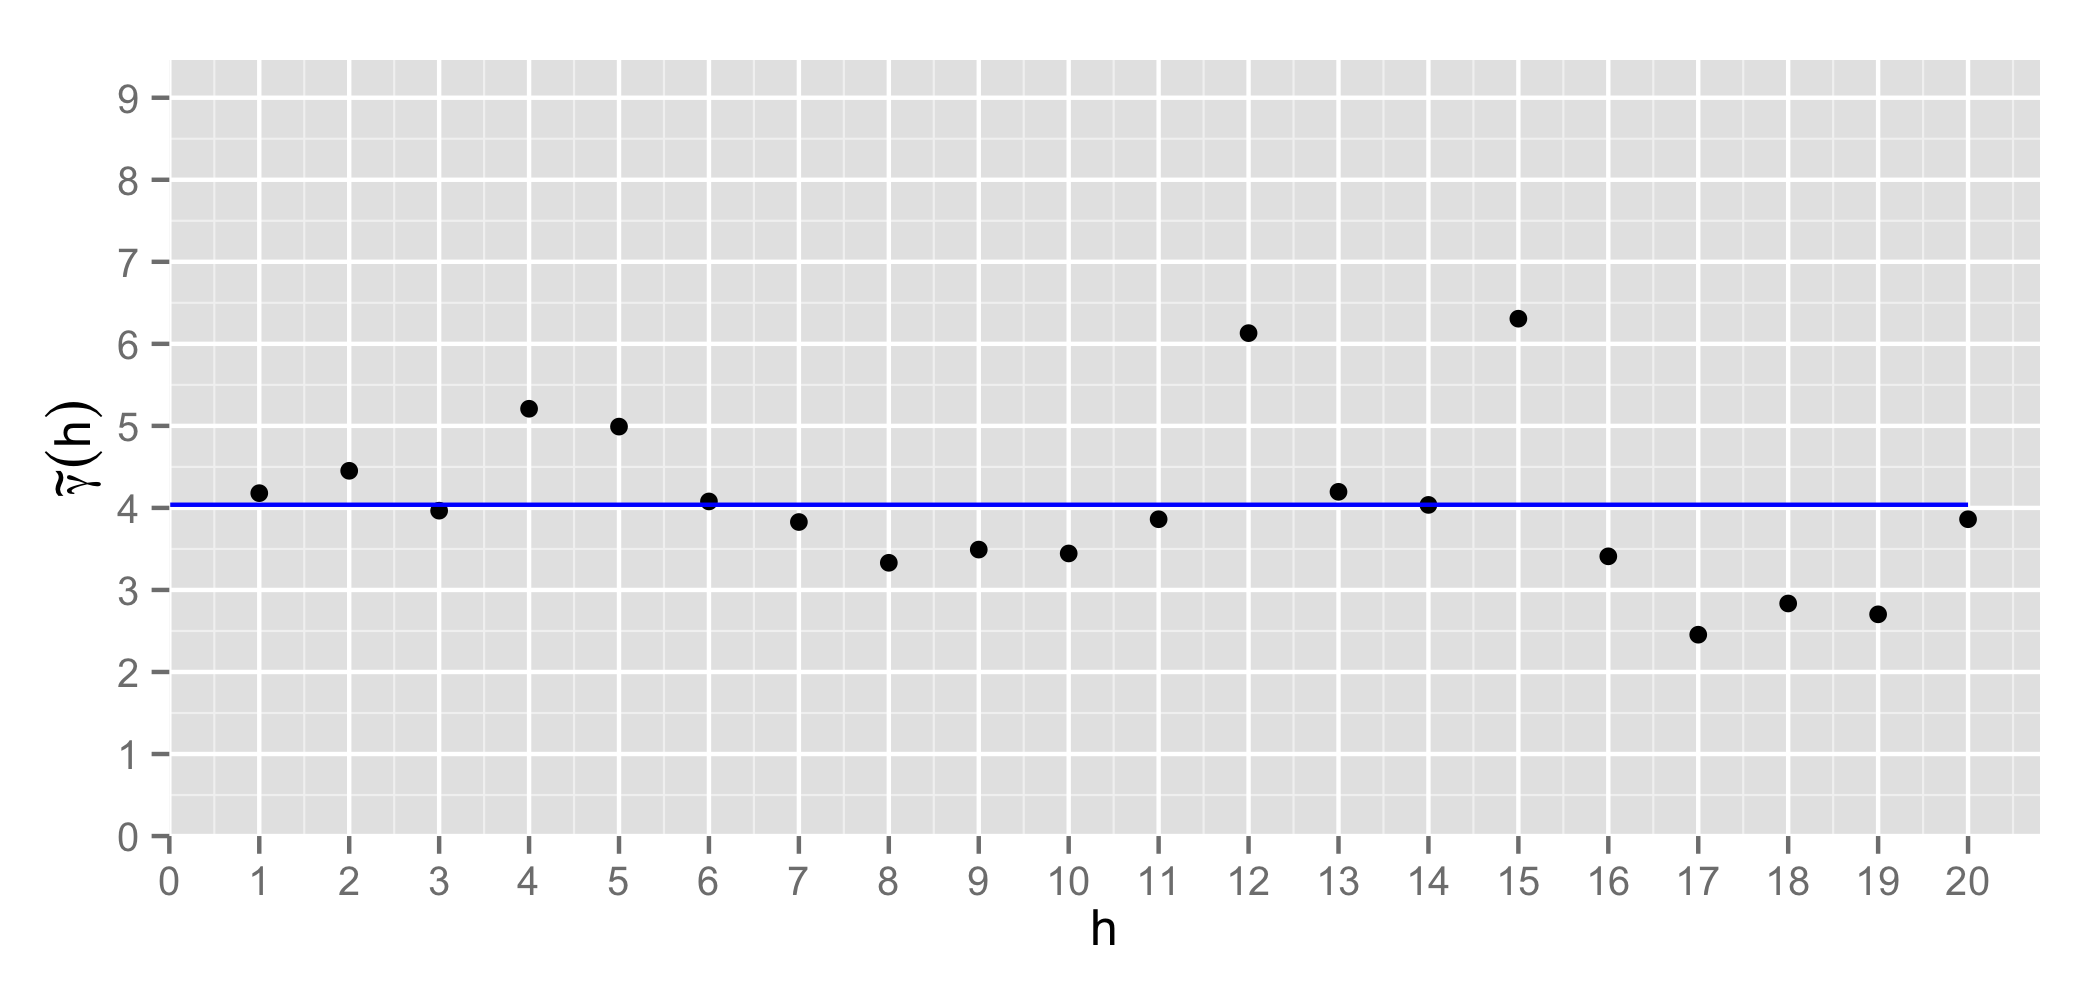
\includegraphics[width=0.9\linewidth]{../../figures/variogram/lin-fit-modeled.png} \\
%     \caption{Модель семивариограммы $\widehat{\gamma}_2(h)$}
%     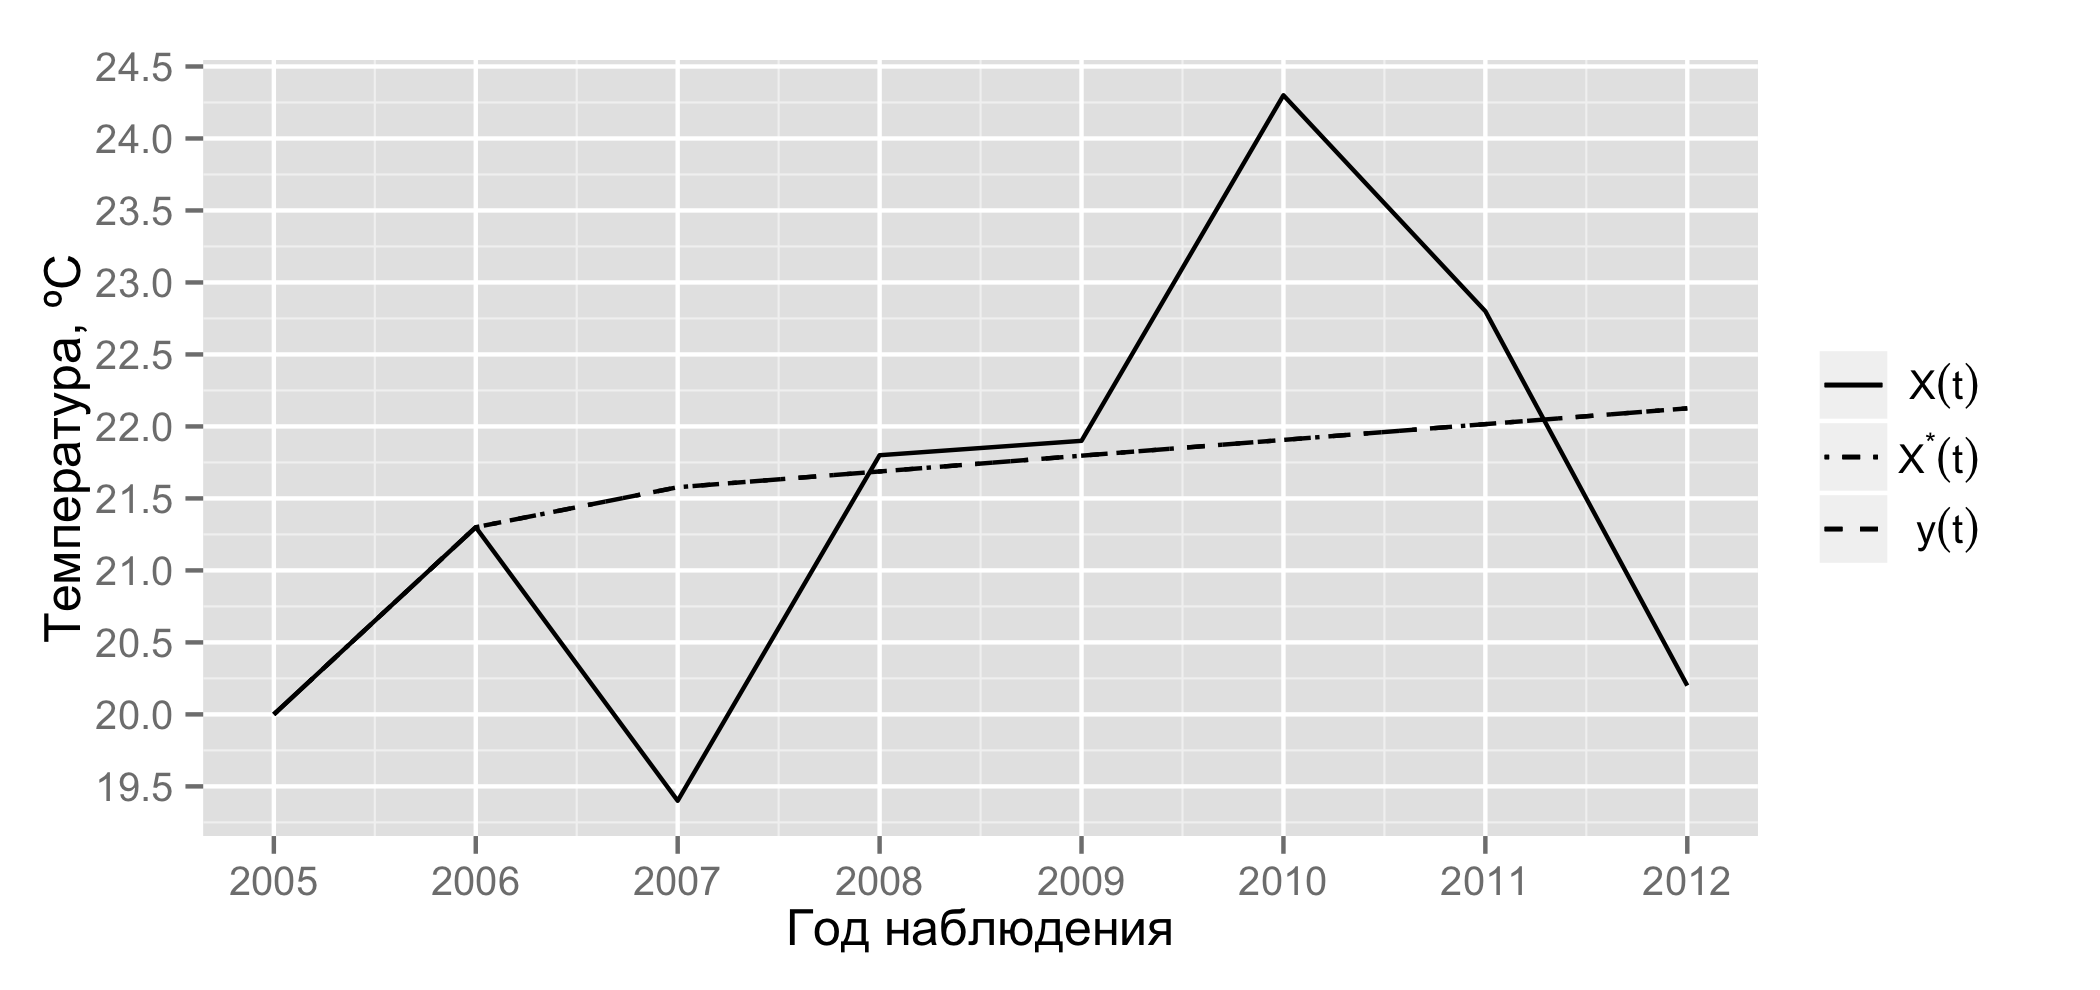
\includegraphics[width=0.9\linewidth]{../../figures/variogram/lin-fit-cross-prediction.png}
%     \caption{Прогноз по модели $\widehat{\gamma}_2(h)$}
%   \end{figure}
%   \end{columns}
% \end{frame}

\begin{frame}
  \frametitle{\large\subsecname}
  \framesubtitle{Линейная модель с порогом}
  \begin{columns}[c]
  \column{0.44\linewidth}
  {\footnotesize
  \begin{equation}\begin{gathered}
  \label{eq:linsill}
    \widehat{\gamma}(h) = c_0 + c \cdot Lin(h, a) = \\
    = \left\{
    \begin{array}{l l}
     c_0 + c \cdot \frac{h}{a}, & 0 \leq h \leq a, \\
     c_0 + c, & h > a,
    \end{array} \right.
  \end{gathered}\end{equation}
  где $ c_0 $ -- эффект самородков, $ c $ -- порог, $ a $ -- ранг.

  \vspace{0.5em}

  Подобранная модель:
  \begin{equation}
  \label{eq:gamma4}
    \widehat{\gamma}_2(h) = 4 \cdot Lin(h, 2).
  \end{equation}

  Показатели качества
  \begin{equation*}
    r_{\varepsilon\varepsilon^{*}} = 0.152, \quad MSE = 18.69
  \end{equation*}
  }

  \column{0.56\linewidth}
  \vspace{-14.5pt}
  \begin{figure}[H]
    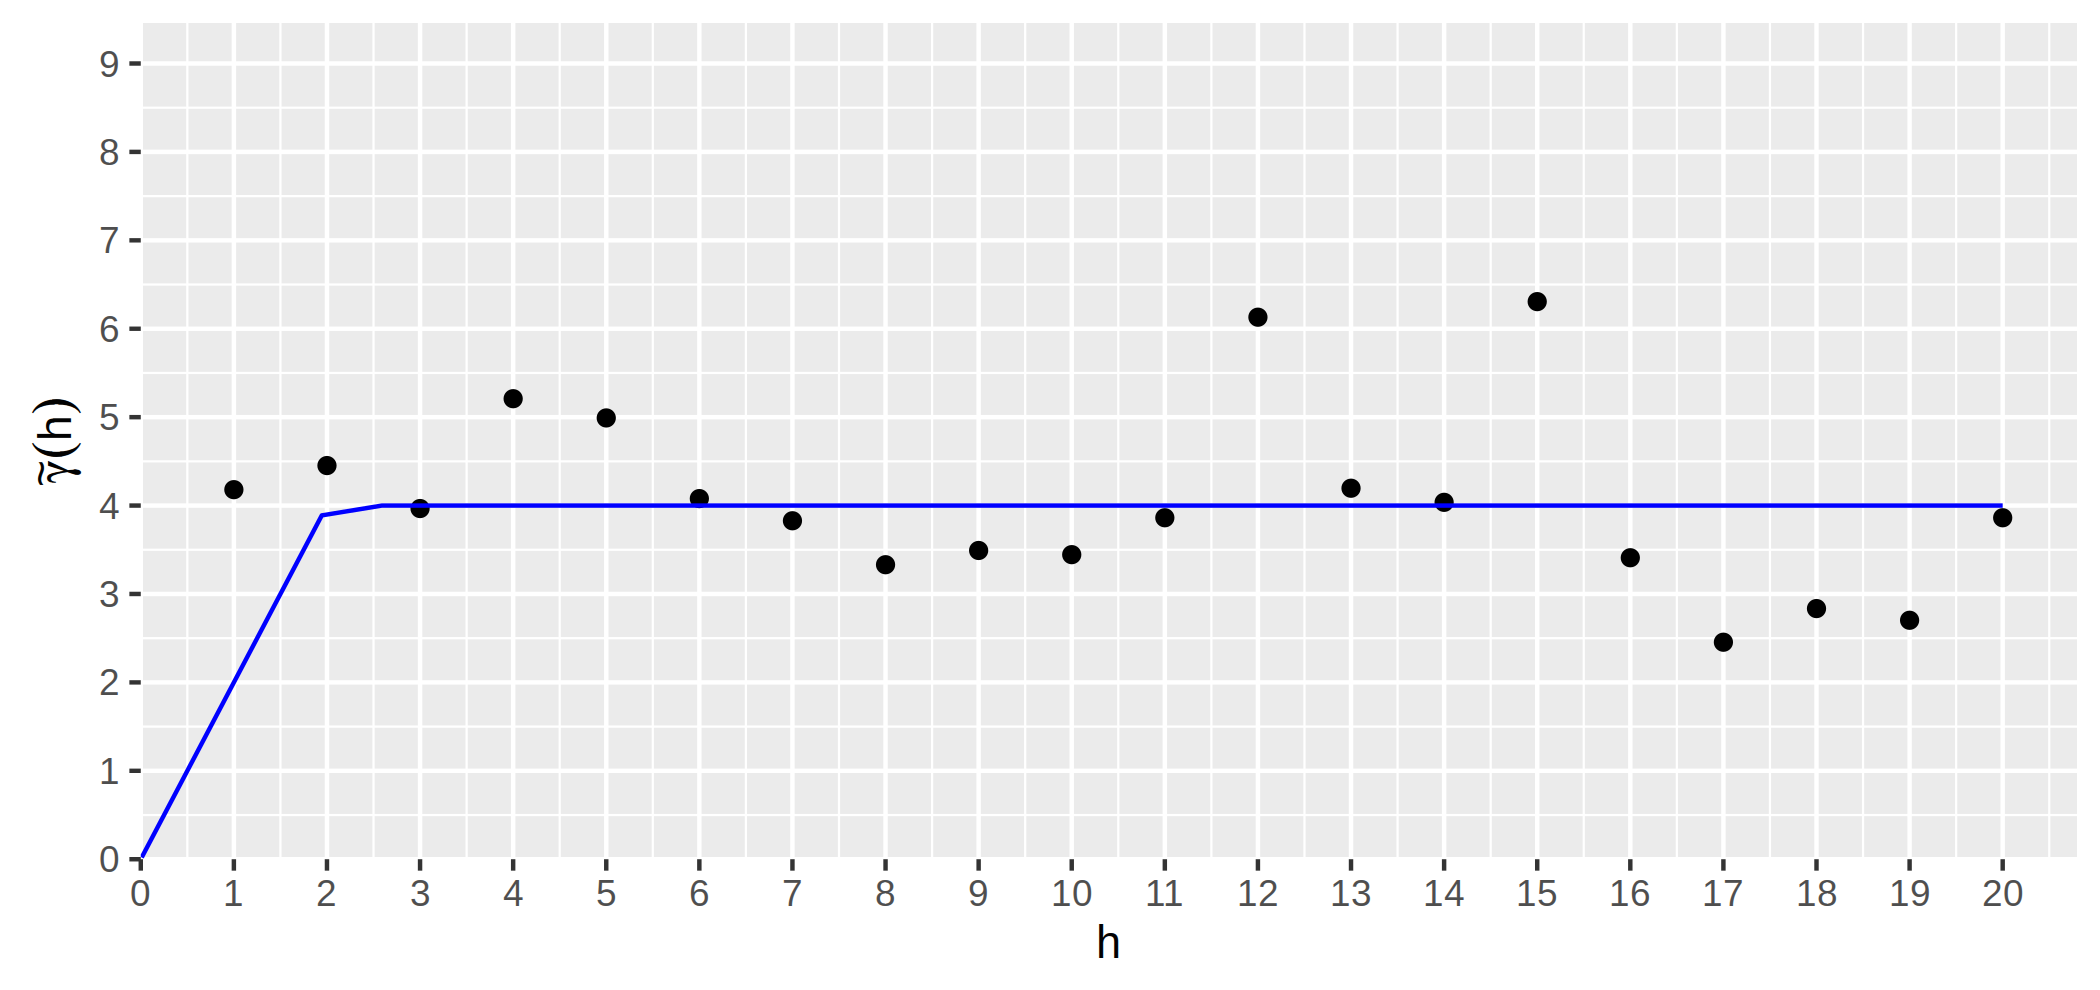
\includegraphics[width=0.9\linewidth]{../../figures/variogram/lin-fit-adapt-modeled.png} \\
    \caption{Модель семивариограммы $\widehat{\gamma}_2(h)$}
    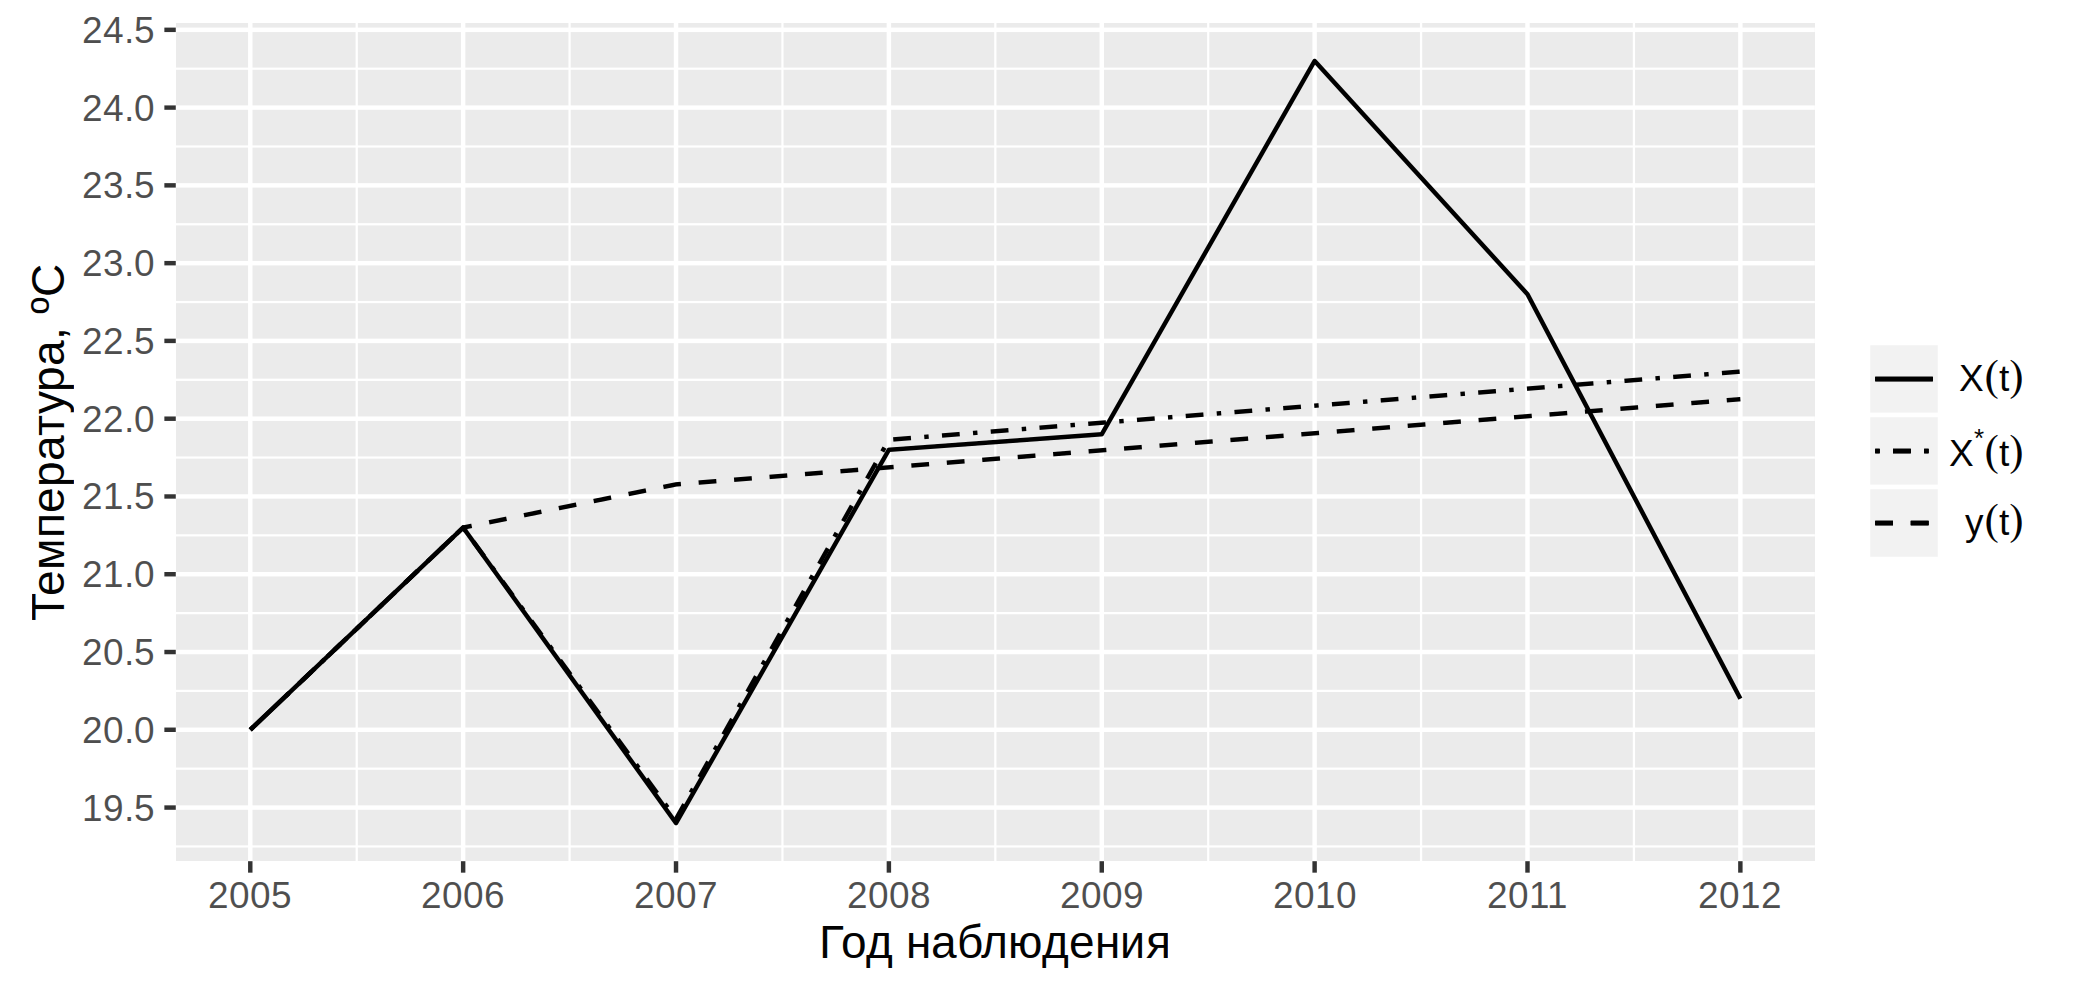
\includegraphics[width=0.9\linewidth]{../../figures/variogram/lin-fit-adapt-cross-prediction.png}
    \caption{Прогноз по модели $\widehat{\gamma}_2(h)$}
  \end{figure}
  \end{columns}
\end{frame}

\begin{frame}
  \frametitle{\large\subsecname}
  \framesubtitle{Сферическая модель}
  \begin{columns}[c]
  \column{0.44\linewidth}
  {\footnotesize
  \begin{equation}\begin{gathered}
  \label{eq:sph}
    \widehat{\gamma}(h) = c_0 + c \cdot Sph(h, a) = \\
    = \left\{
    \begin{array}{l l}
      c_0 + c \cdot (\frac{3}{2} \frac{h}{a} - \frac{1}{2}(\frac{h}{a})^3), & h \le a, \\
      c_0 + c, & h \geq a,
    \end{array} \right.
  \end{gathered}\end{equation}
  где $ c_0 $ -- эффект самородков, $ c $ -- порог, $ a $ -- ранг.

  \vspace{0.5em}

  Подобранная модель:
  \begin{equation}
  \label{eq:gamma5}
    \widehat{\gamma}_3(h) = 0.9 + 4 Sph(h, 6.9),
  \end{equation}

  Показатели качества
  \begin{equation*}
    r_{\varepsilon\varepsilon^{*}} = -0.009, \quad MSE = 5.396
  \end{equation*}
  }

  \column{0.56\linewidth}
  \vspace{-14.5pt}
  \begin{figure}[H]
    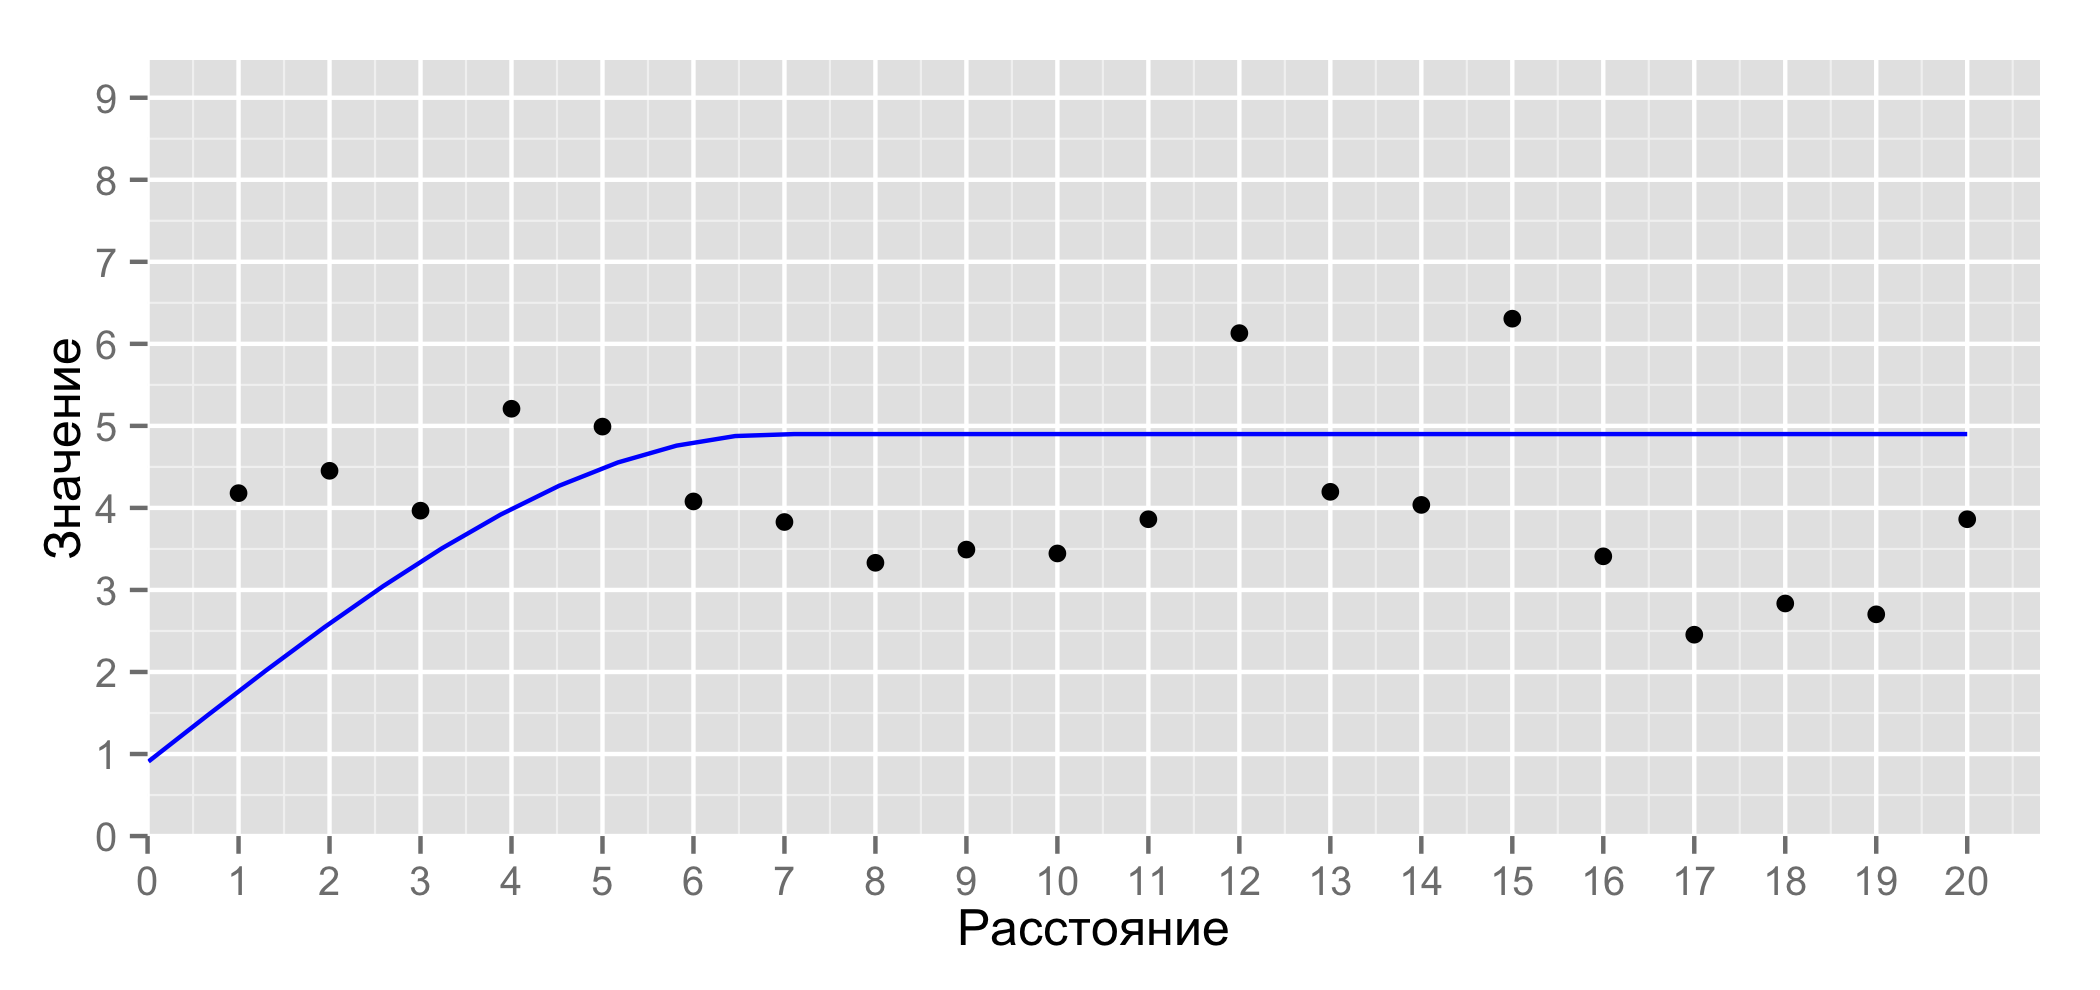
\includegraphics[width=0.9\linewidth]{../../figures/variogram/sph-fit-adapt-modeled.png} \\
    \caption{Модель семивариограммы $\widehat{\gamma}_3(h)$}
    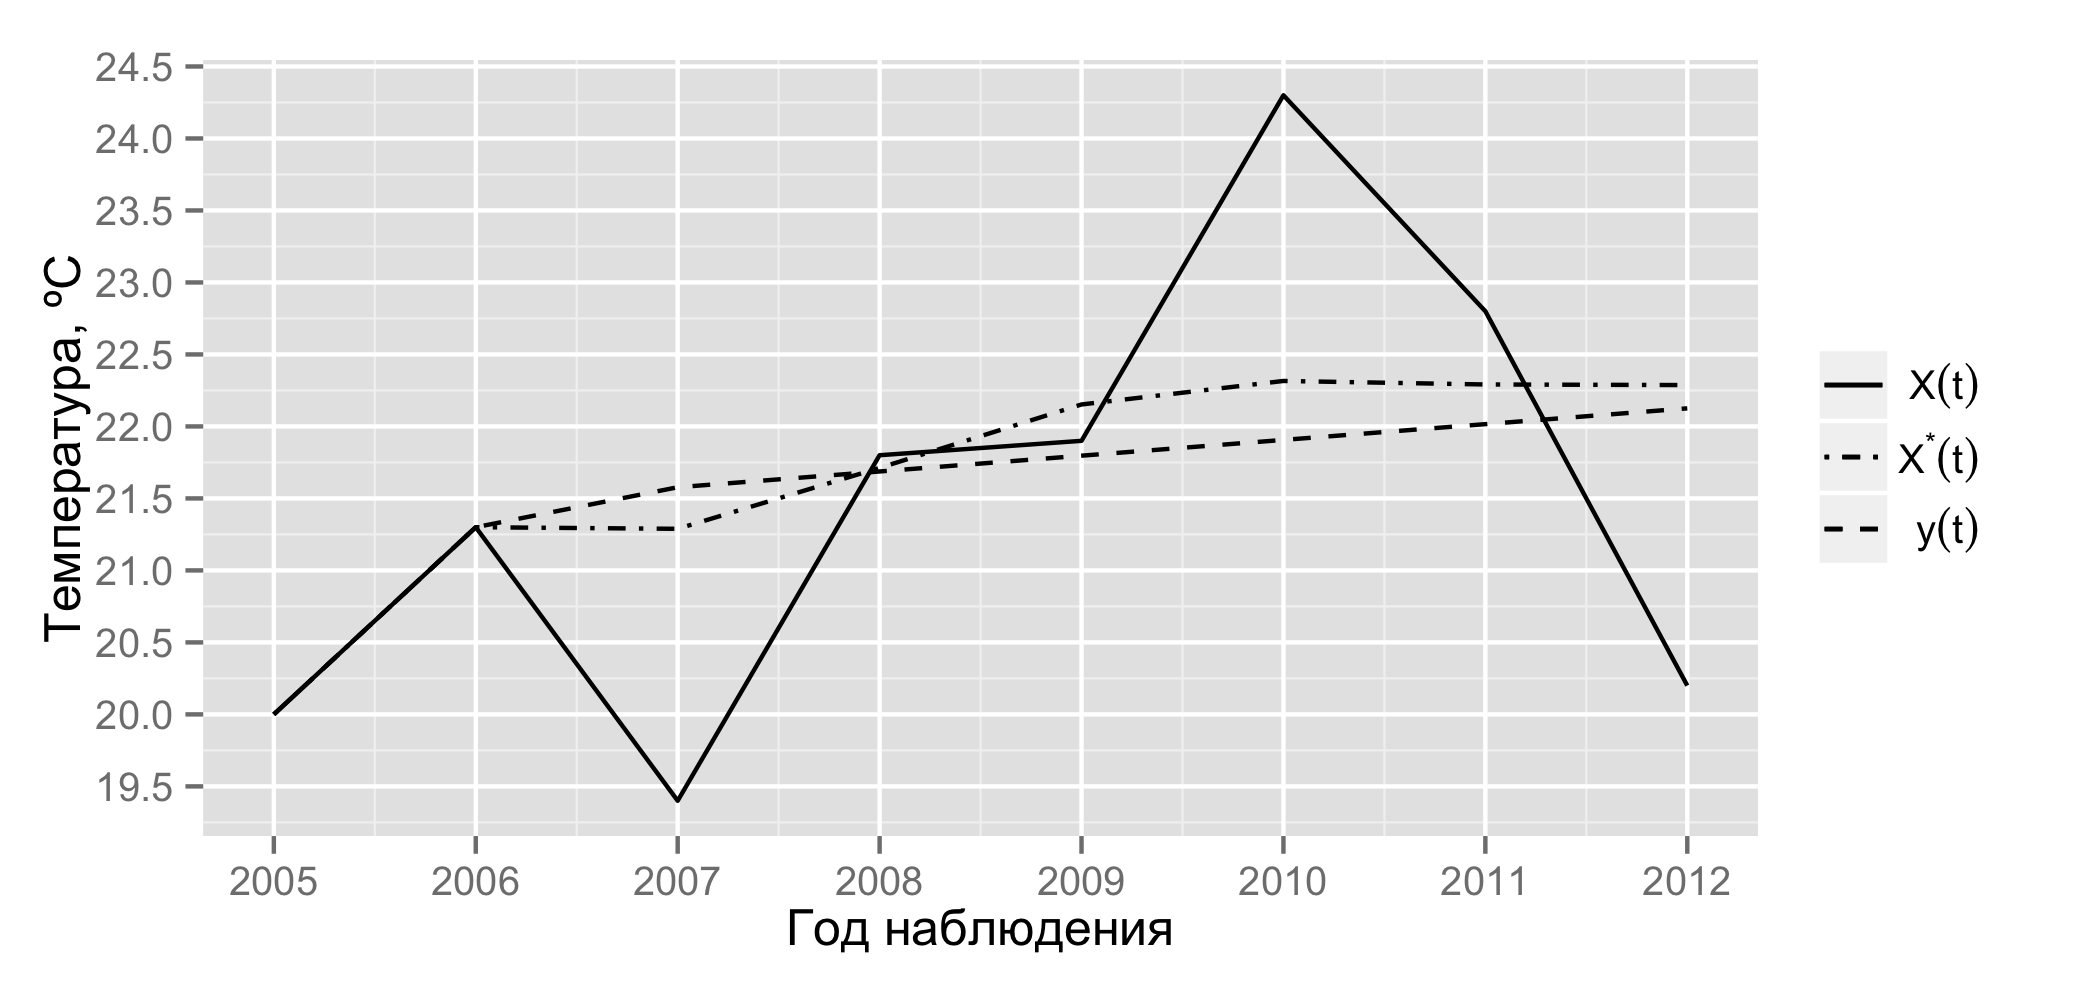
\includegraphics[width=0.9\linewidth]{../../figures/variogram/sph-fit-adapt-cross-prediction.png}
    \caption{Прогноз по модели $\widehat{\gamma}_3(h)$}
  \end{figure}
  \end{columns}
\end{frame}

\begin{frame}
  \frametitle{\large\subsecname}
  \framesubtitle{Периодическая модель}
  \begin{columns}[c]
  \column{0.44\linewidth}
  {\footnotesize
  \begin{eqnarray}
  \label{eq:per}
    \widehat{\gamma}(h) = c_0 + c \cdot Per(h, a) = \nonumber \\
    = 1 - cos(\frac{2 \pi h}{a}),
  \end{eqnarray}
  где $ c_0 $ -- эффект самородков, $ c $ -- порог, $ a $ -- ранг.

  \vspace{0.5em}

  Подобранная модель:
  \begin{equation}
  \label{eq:gamma6}
    \widehat{\gamma}_4(h) = 4 \cdot Per(h, 0.898),
  \end{equation}

  Показатели качества
  \begin{equation*}
    r_{\varepsilon\varepsilon^{*}} = 0.404, \quad MSE = 4.369
  \end{equation*}
  }

  \column{0.56\linewidth}
  \vspace{-14.5pt}
  \begin{figure}[H]
    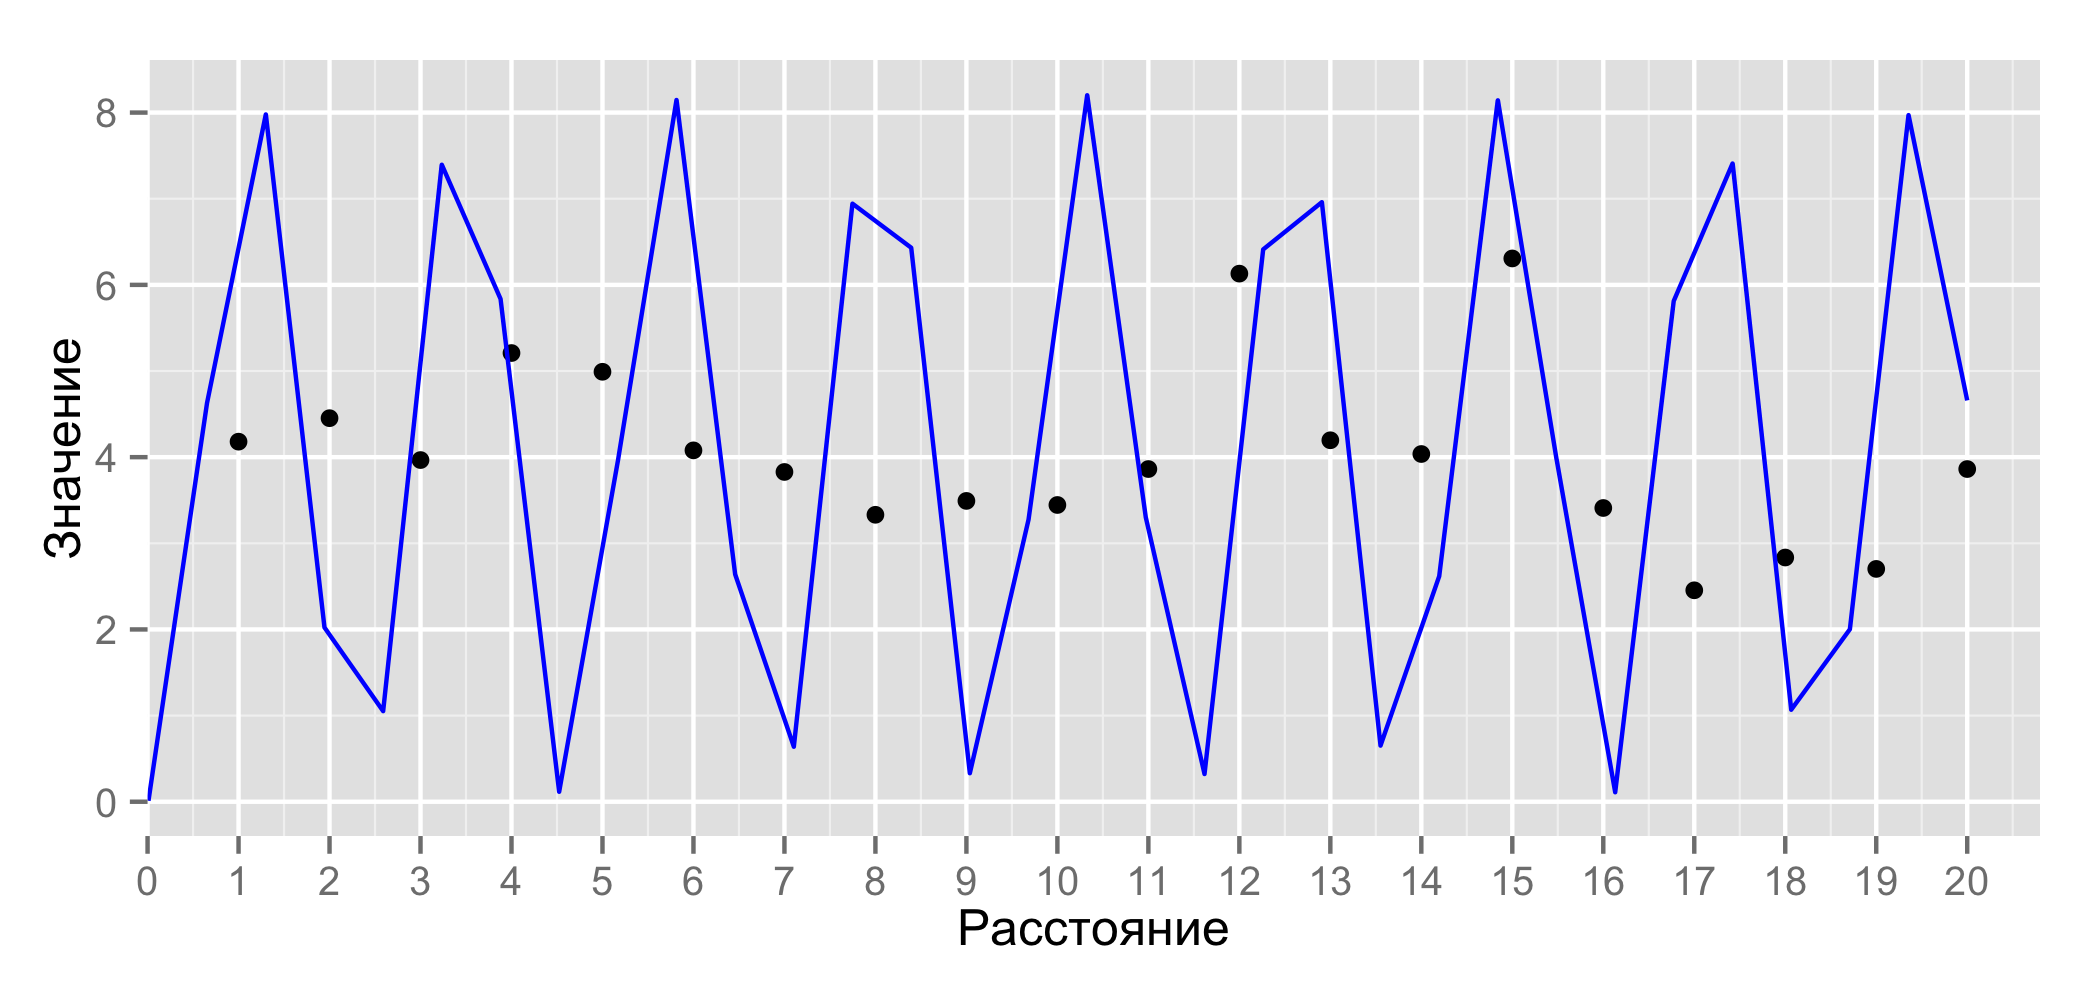
\includegraphics[width=0.9\linewidth]{../../figures/variogram/per-fit-cv-modeled.png} \\
    \caption{Модель семивариограммы $\widehat{\gamma}_4(h)$}
    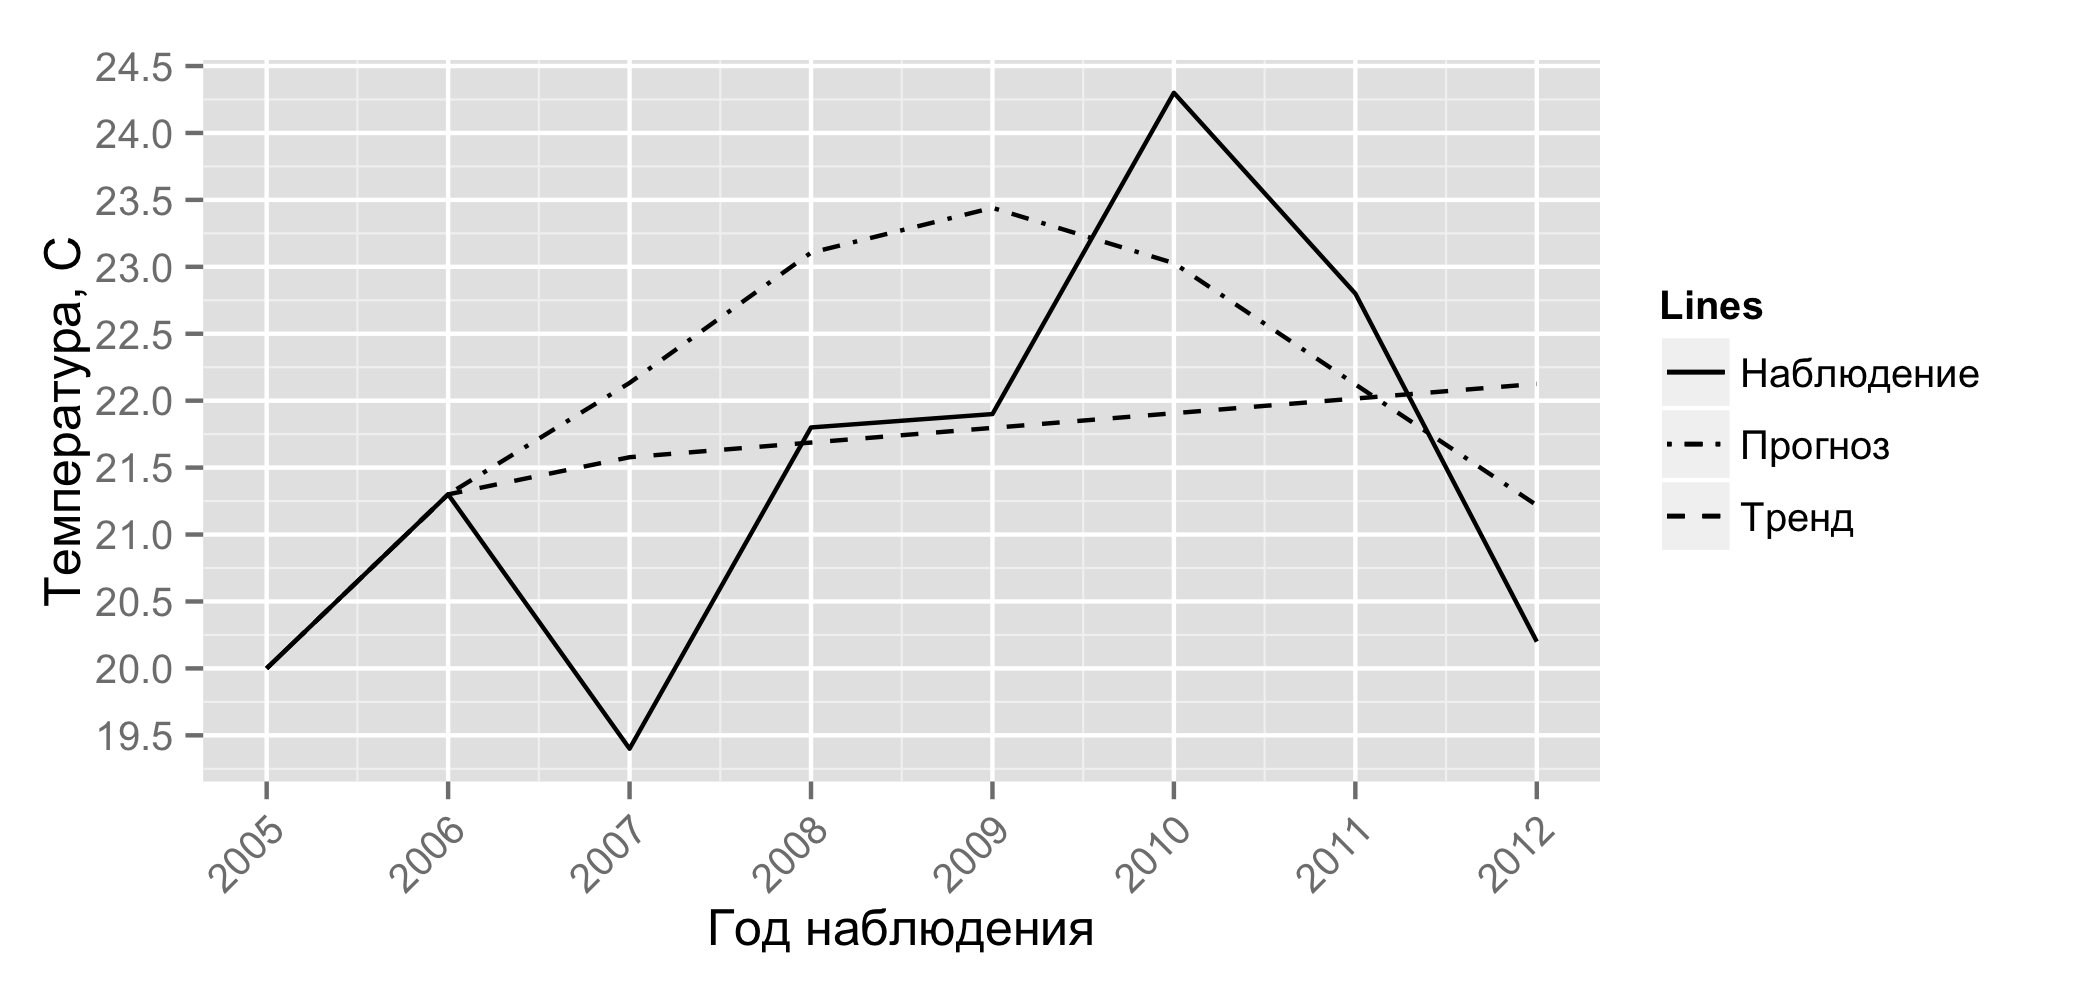
\includegraphics[width=0.9\linewidth]{../../figures/variogram/per-fit-cv-cross-prediction.png}
    \caption{Прогноз по модели $\widehat{\gamma}_4(h)$}
  \end{figure}
  \end{columns}
\end{frame}

\subsection{Автоматический подход}

%\begin{frame}
%  \frametitle{\large\subsecname}
%  \framesubtitle{Оценки семивариограммы}
%  \begin{figure}[h]
%    \begin{minipage}[h]{0.49\linewidth}
%      \center{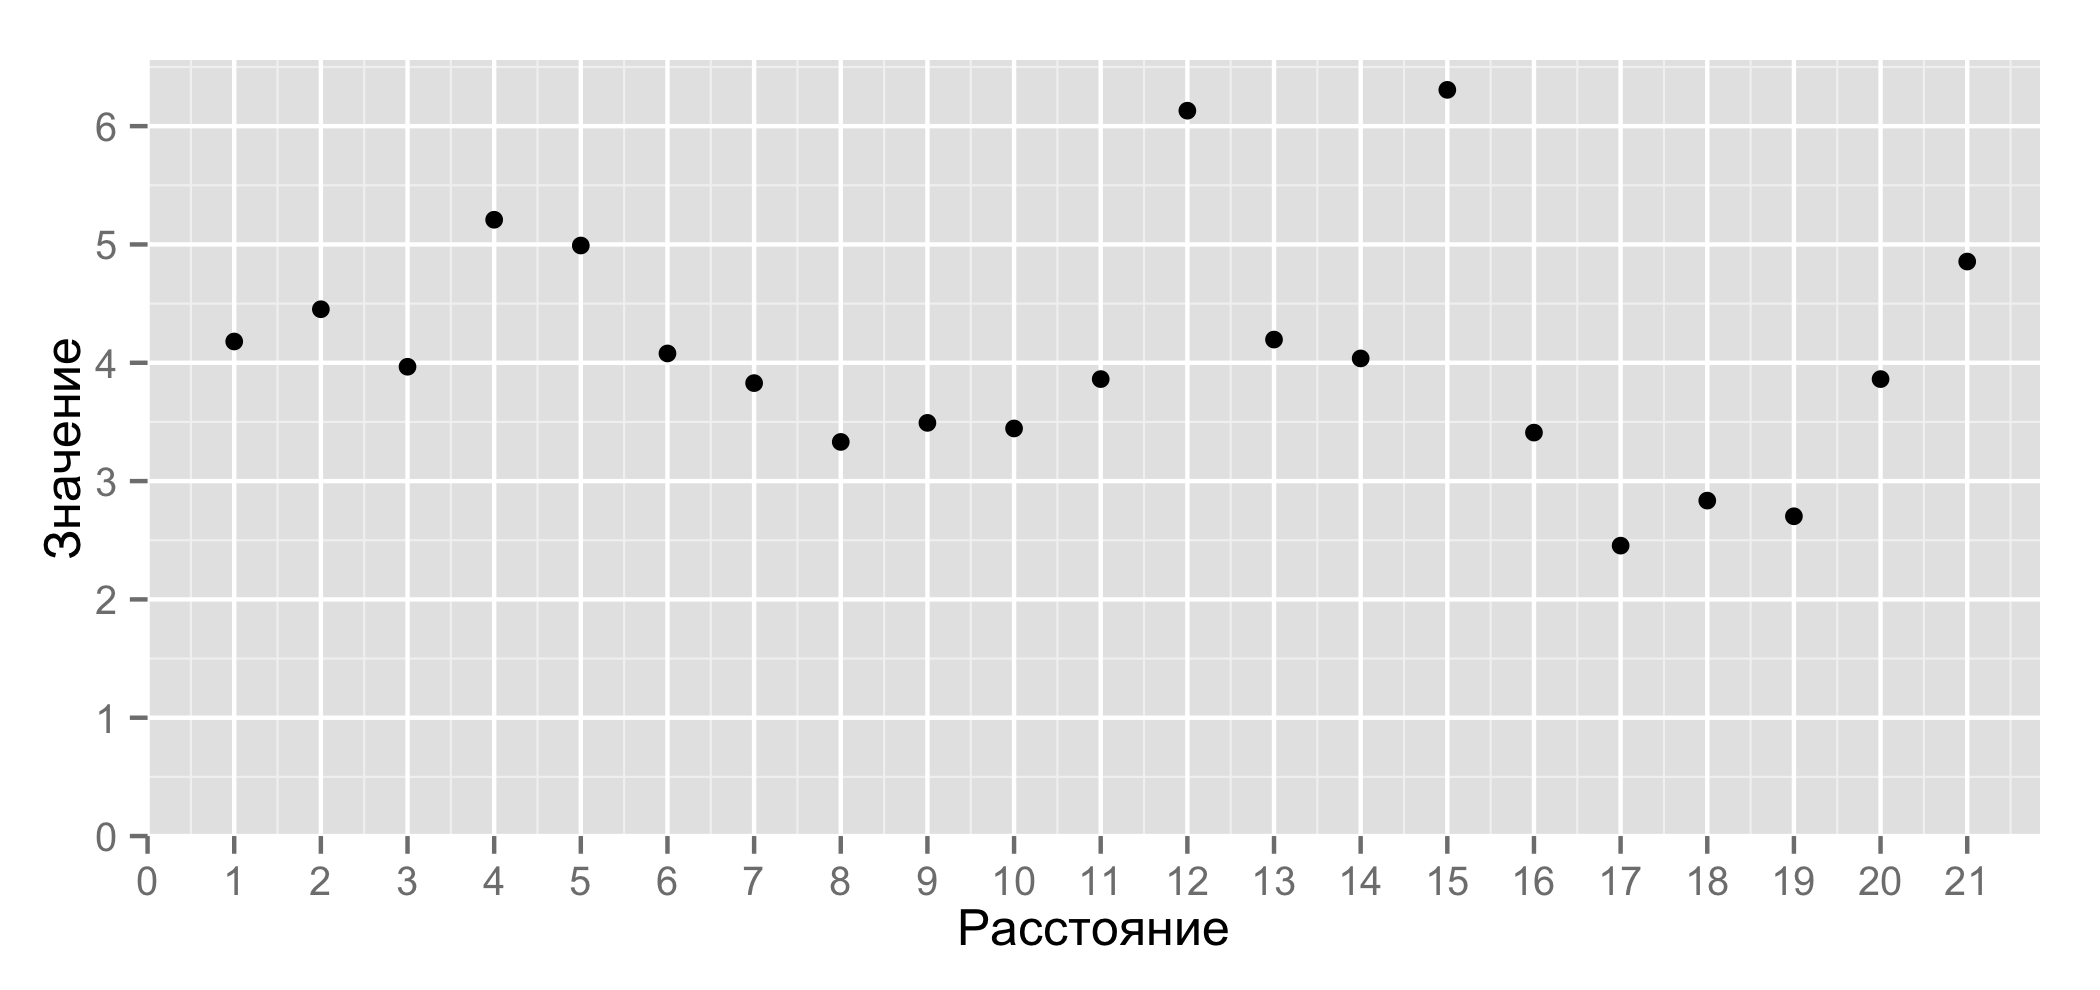
\includegraphics[width=1\linewidth]{../../figures/variogram/lin-variogram.png}}
%      \caption{Оценка Матерона}
%    \end{minipage}
%    \hfill
%    \begin{minipage}[h]{0.49\linewidth}
%      \center{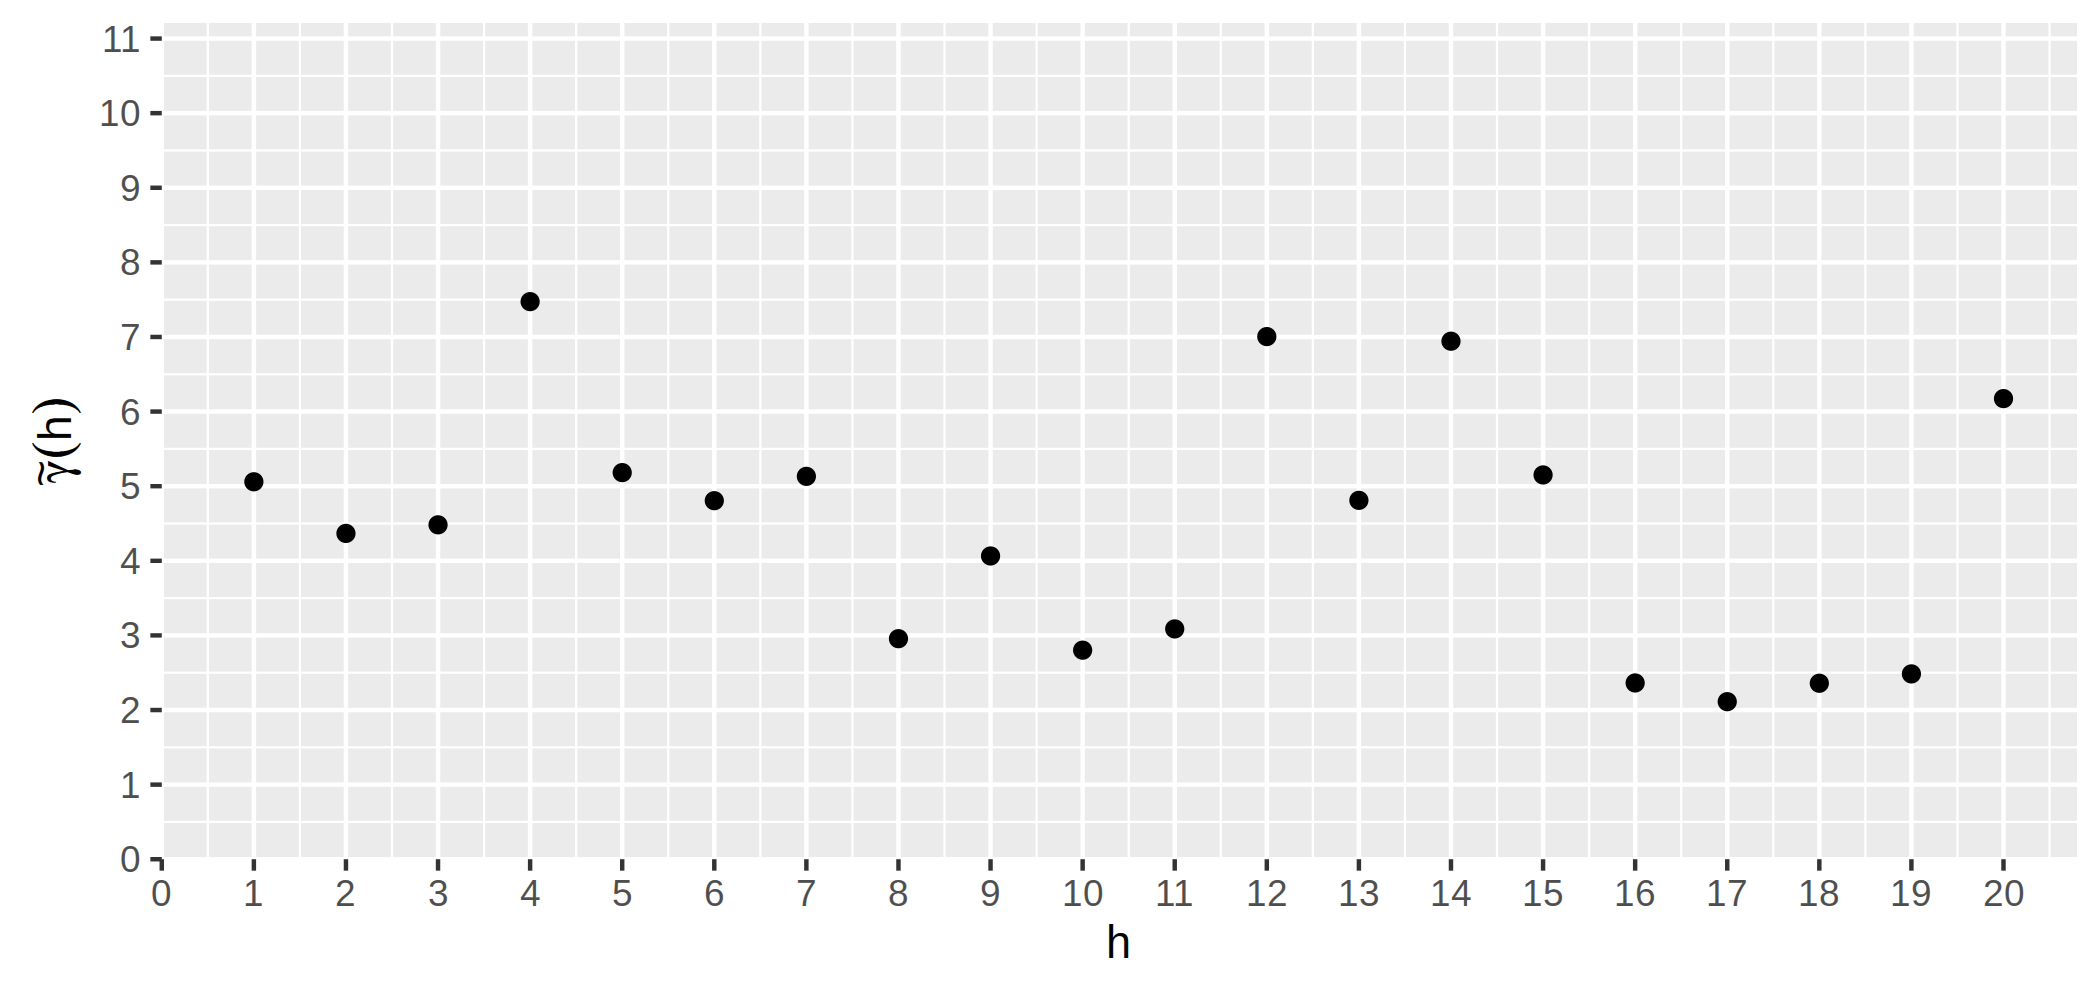
\includegraphics[width=1\linewidth]{../../figures/variogram/robust-variogram.png}}
%      \caption{Оценка Кресси-Хоккинса}
%    \end{minipage}
%  \end{figure}
%  Робастная оценка семивариограммы Кресси-Хокинса:
%  \begin{equation}
%  \label{eq:cressie}
%    2 \tilde{\gamma}(h) = \frac{1}{n - h} (\sum_{t = 1}^{n - h} | X(t + h) - X(t) |^{\frac{1}{2}} )^4 / (0.457 + \frac{0.494}{n - h} + \frac{0.045}{(n - h)^2}), \quad h = \overline{0, n - 1}.
%  \end{equation}
%\end{frame}

\begin{frame}
  \frametitle{\large\subsecname}
  \framesubtitle{Периодическая модель}
  \begin{columns}[c]
  \column{0.44\linewidth}
  {\footnotesize
  \begin{equation*}
    \widehat{\gamma}(h) = c_0 + c \cdot Per(h, a) = 1 - cos(\frac{2 \pi h}{a}),
  \end{equation*}
  где $ c_0 $ -- эффект самородков, $ c $ -- порог, $ a $ -- ранг.

  \vspace{0.5em}

  Подобранная модель:
  \begin{equation}
  \label{eq:gamma10}
    \widehat{\gamma}_5(h) = 3.8 + 0.32 \cdot Per(h, 1.3)
  \end{equation}

  Показатели качества
  \begin{equation*}
    r_{\varepsilon\varepsilon^{*}} = 0.11, \quad MSE = 5.22
  \end{equation*}
  }

  \column{0.56\linewidth}
  \vspace{-14.5pt}
  \begin{figure}[H]
    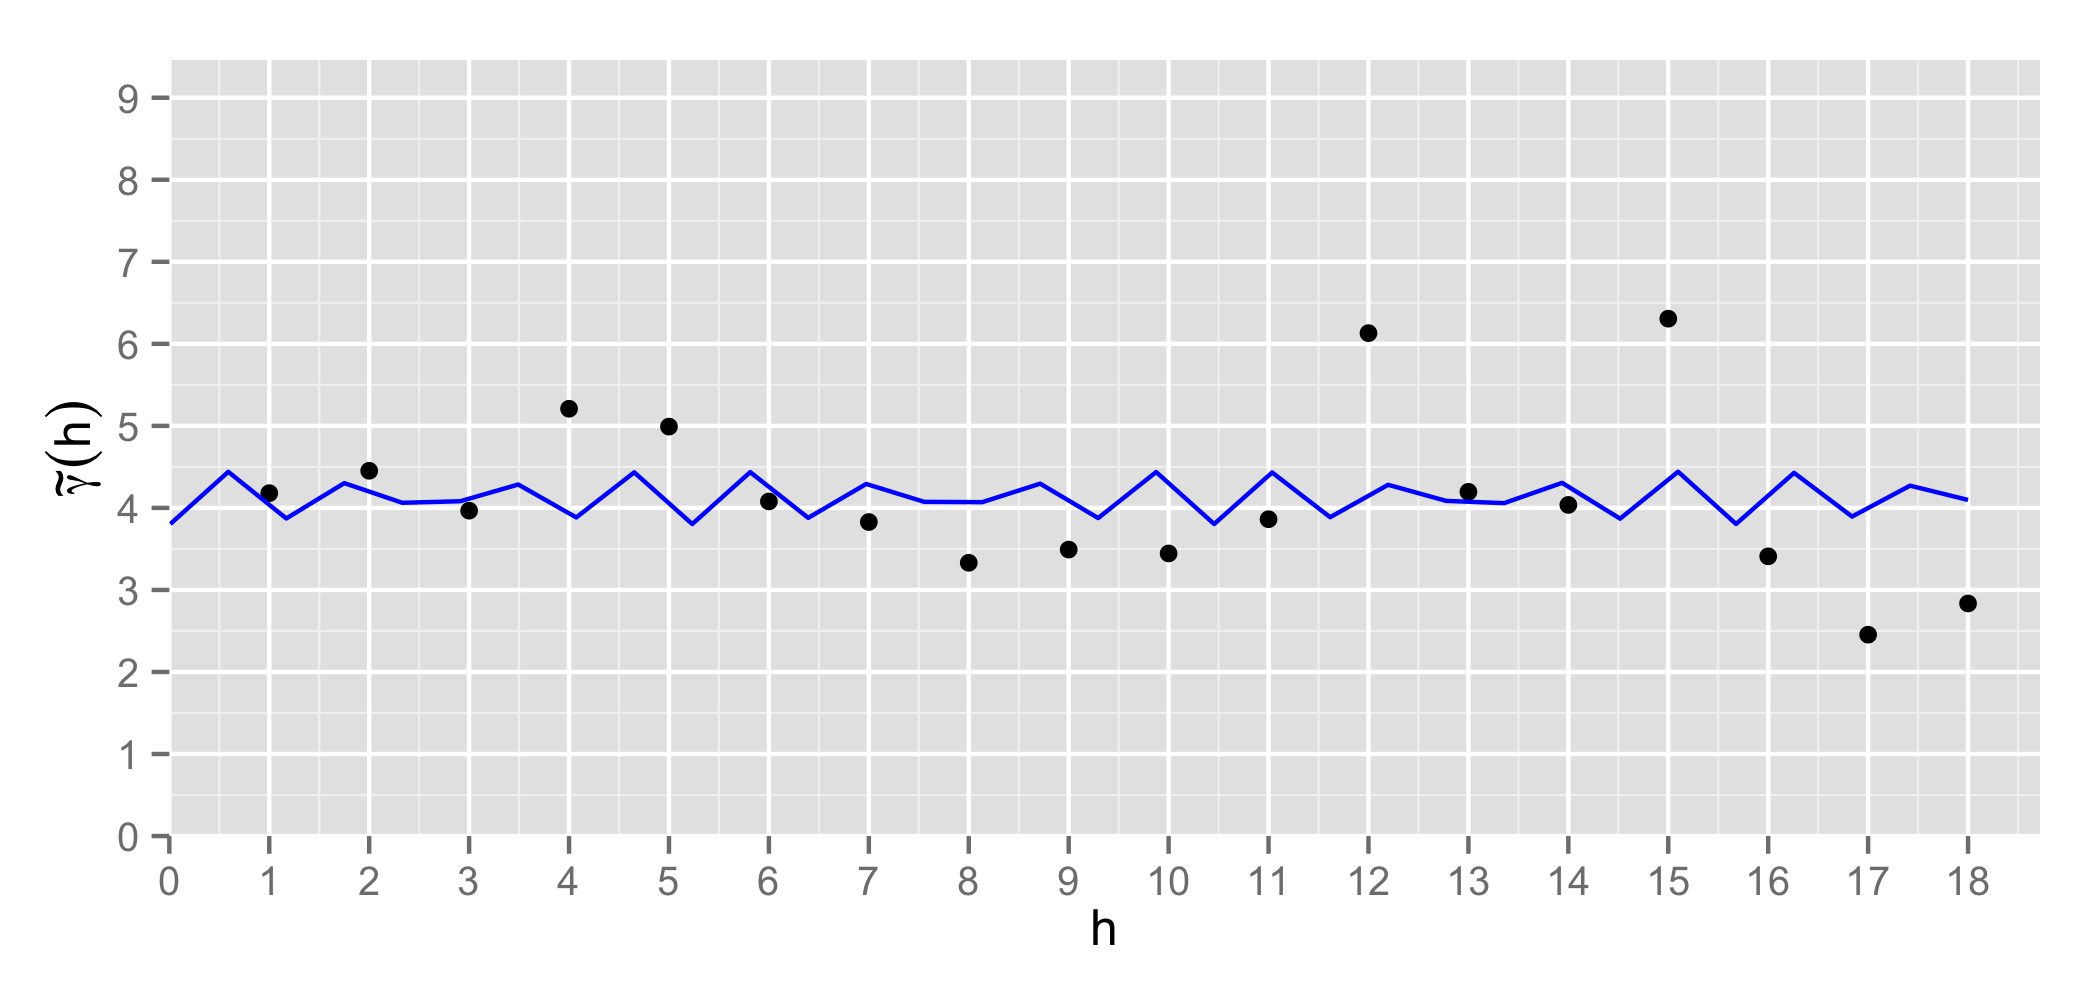
\includegraphics[width=0.9\linewidth]{../../figures/variogram/auto-class-18-modeled.png} \\
    \caption{Модель семивариограммы $\widehat{\gamma}_5(h)$}
    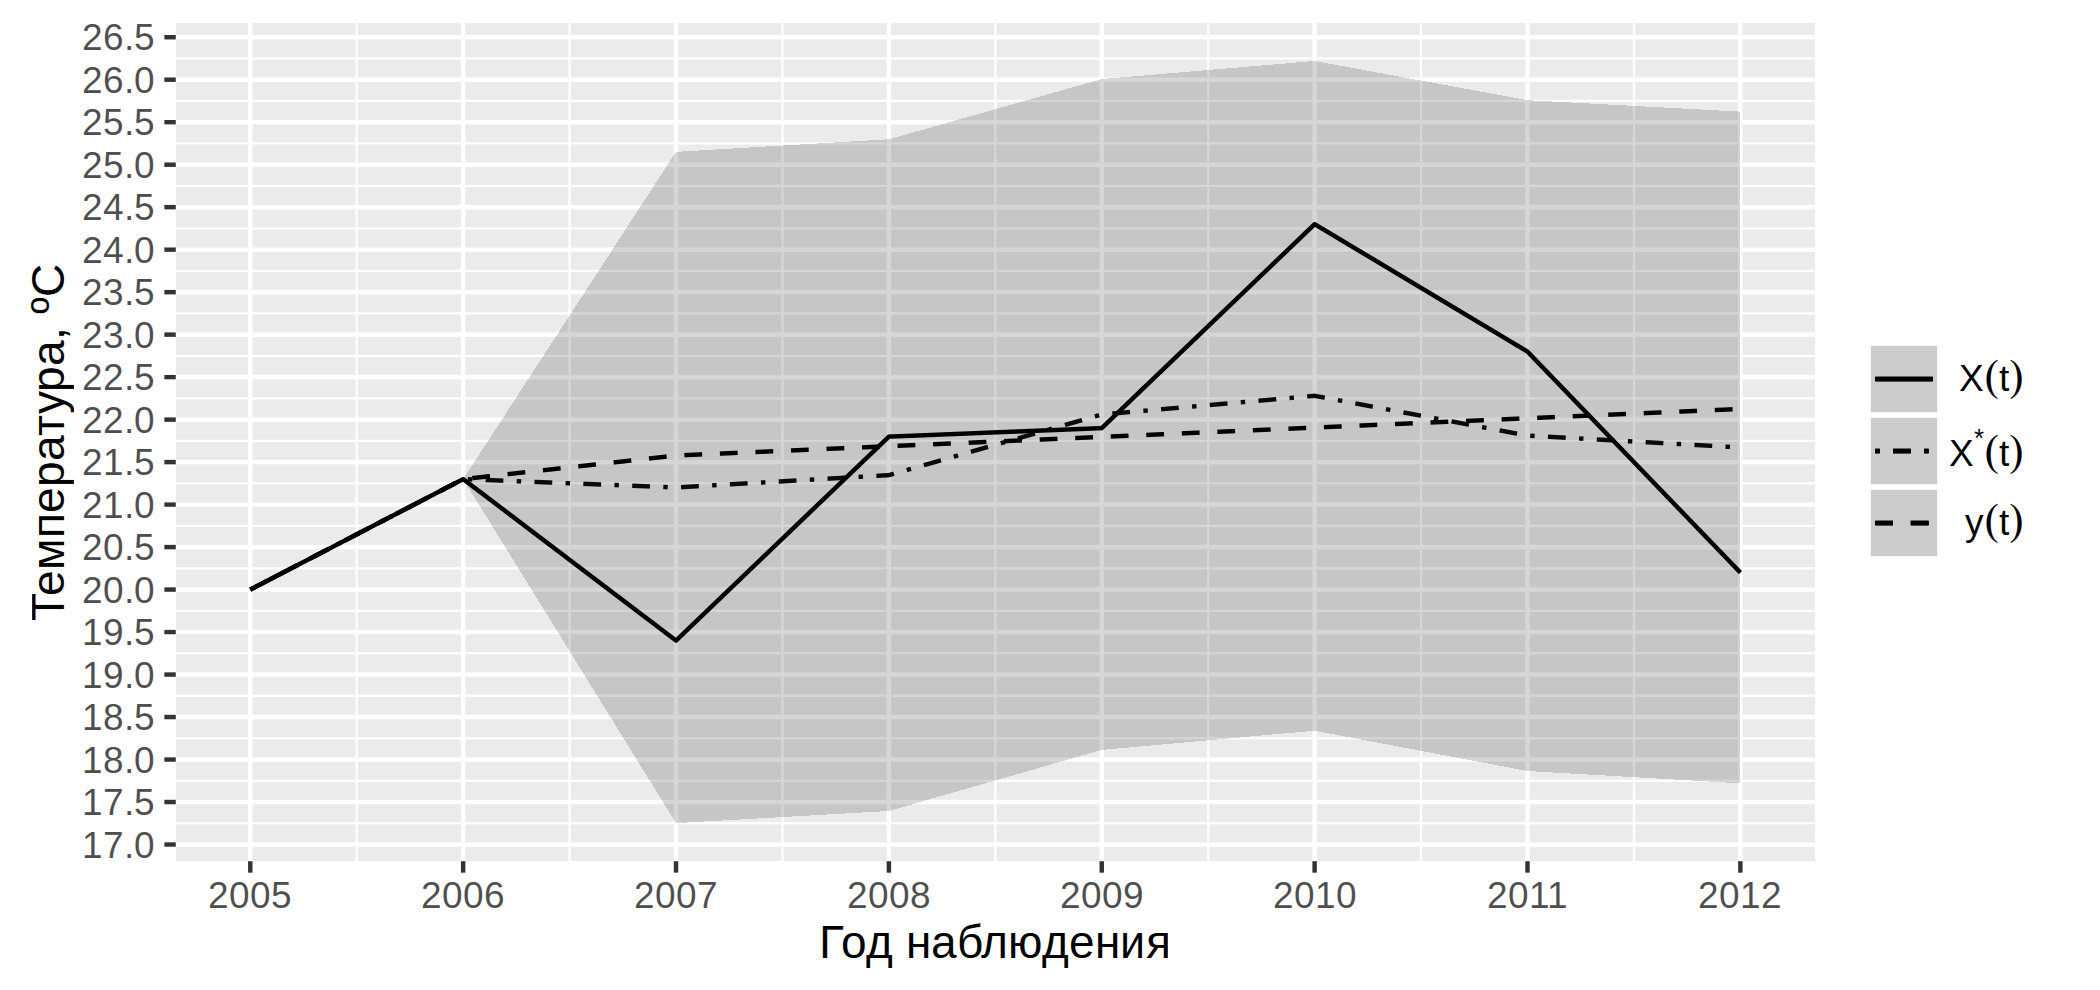
\includegraphics[width=0.9\linewidth]{../../figures/variogram/auto-class-18-cross-prediction.png}
    \caption{Прогноз по модели $\widehat{\gamma}_5(h)$}
  \end{figure}
  \end{columns}
\end{frame}

\begin{frame}
  \frametitle{\large\subsecname}
  \framesubtitle{Волновая модель}
  \begin{columns}[c]
  \column{0.44\linewidth}
  {\footnotesize
  \begin{eqnarray}
  \label{eq:wave}
    \widehat{\gamma}(h) = c_0 + c \cdot Wav(h, a) = \nonumber \\
    = 1 - \frac{a}{h} \cdot sin(\frac{h}{a}),
  \end{eqnarray}
  где $ c_0 $ -- эффект самородков, $ c $ -- порог, $ a $ -- ранг.

  \vspace{0.5em}

  Подобранная модель:
  \begin{equation}
  \label{eq:gamma9}
    \widehat{\gamma}_6(h) = 4.11 + 1.65 \cdot Wav(h, 3.59),
  \end{equation}

  Показатели качества
  \begin{equation*}
    r_{\varepsilon\varepsilon^{*}} = -0.03, \quad MSE = 4.20
  \end{equation*}
  }

  \column{0.56\linewidth}
  \vspace{-14.5pt}
  \begin{figure}[H]
    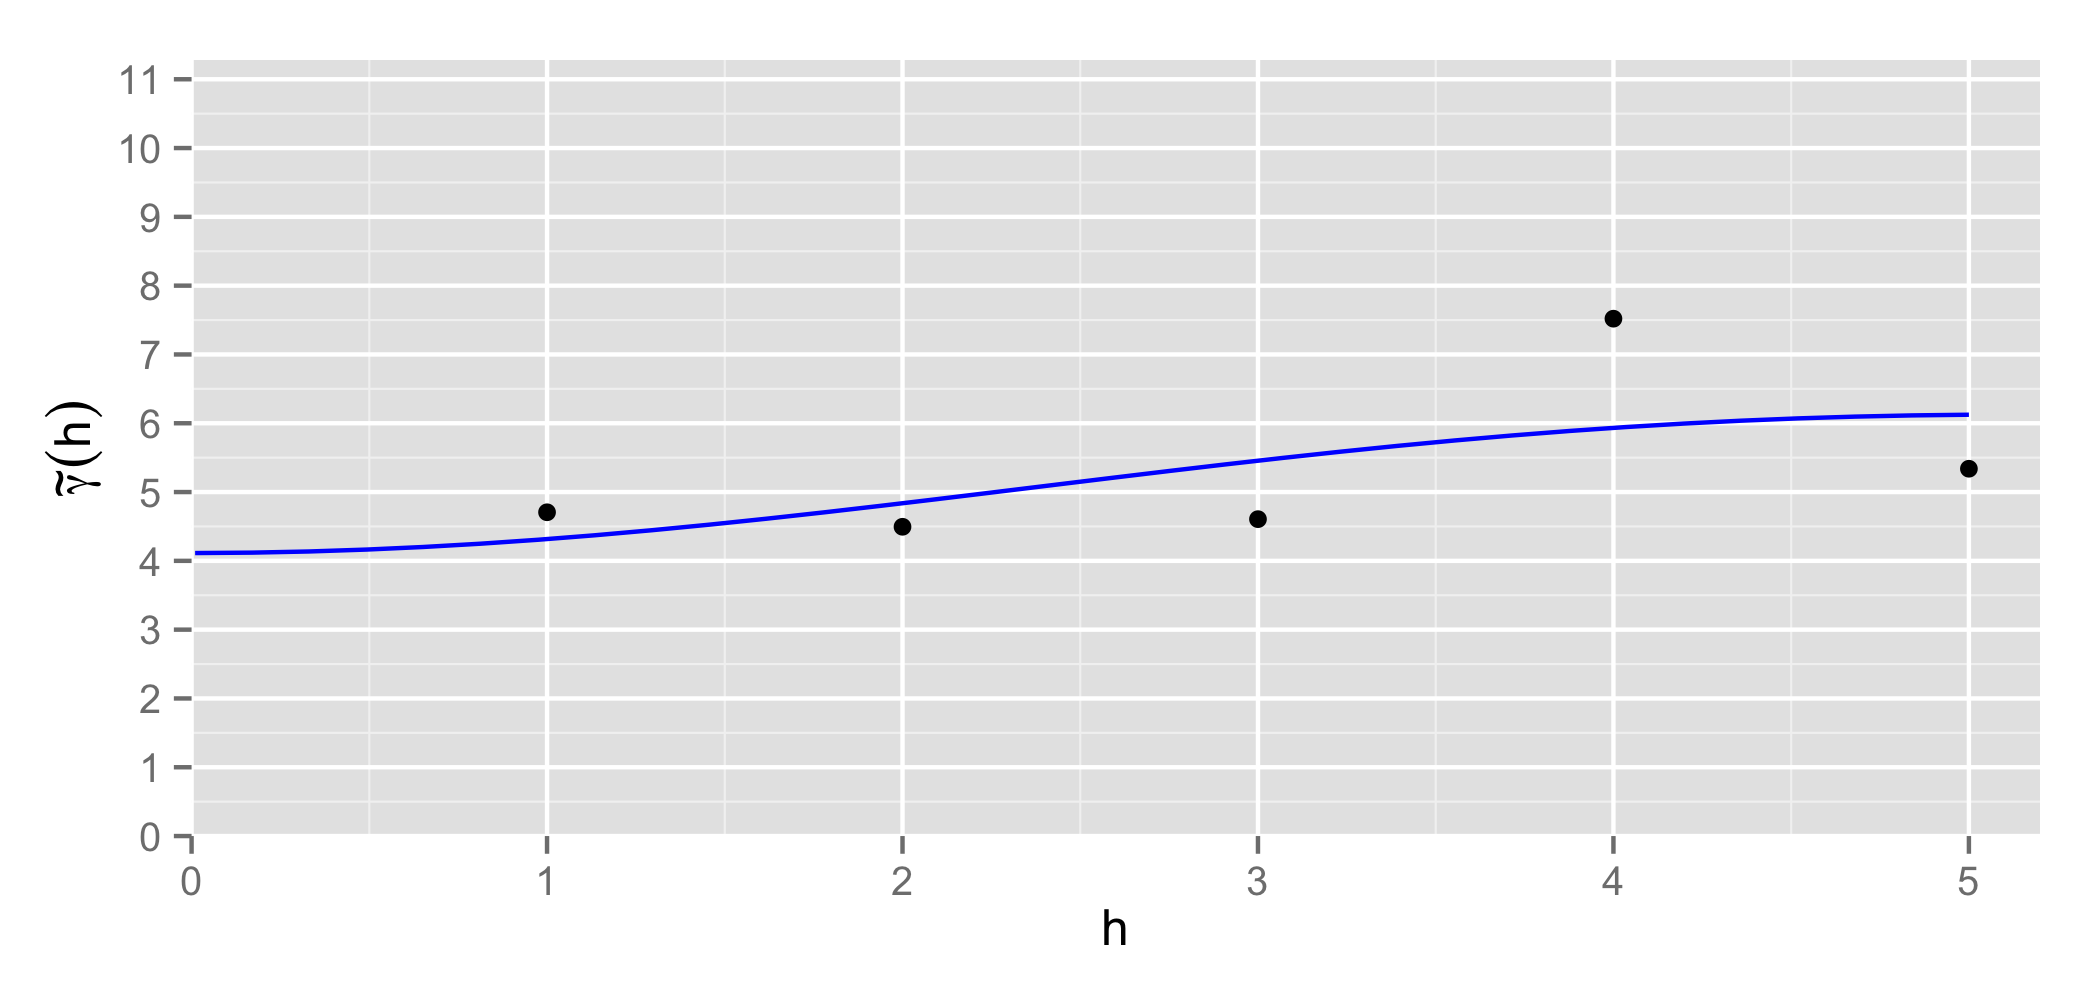
\includegraphics[width=0.9\linewidth]{../../figures/variogram/auto-rob-5-modeled.png} \\
    \caption{Модель семивариограммы $\widehat{\gamma}_6(h)$}
    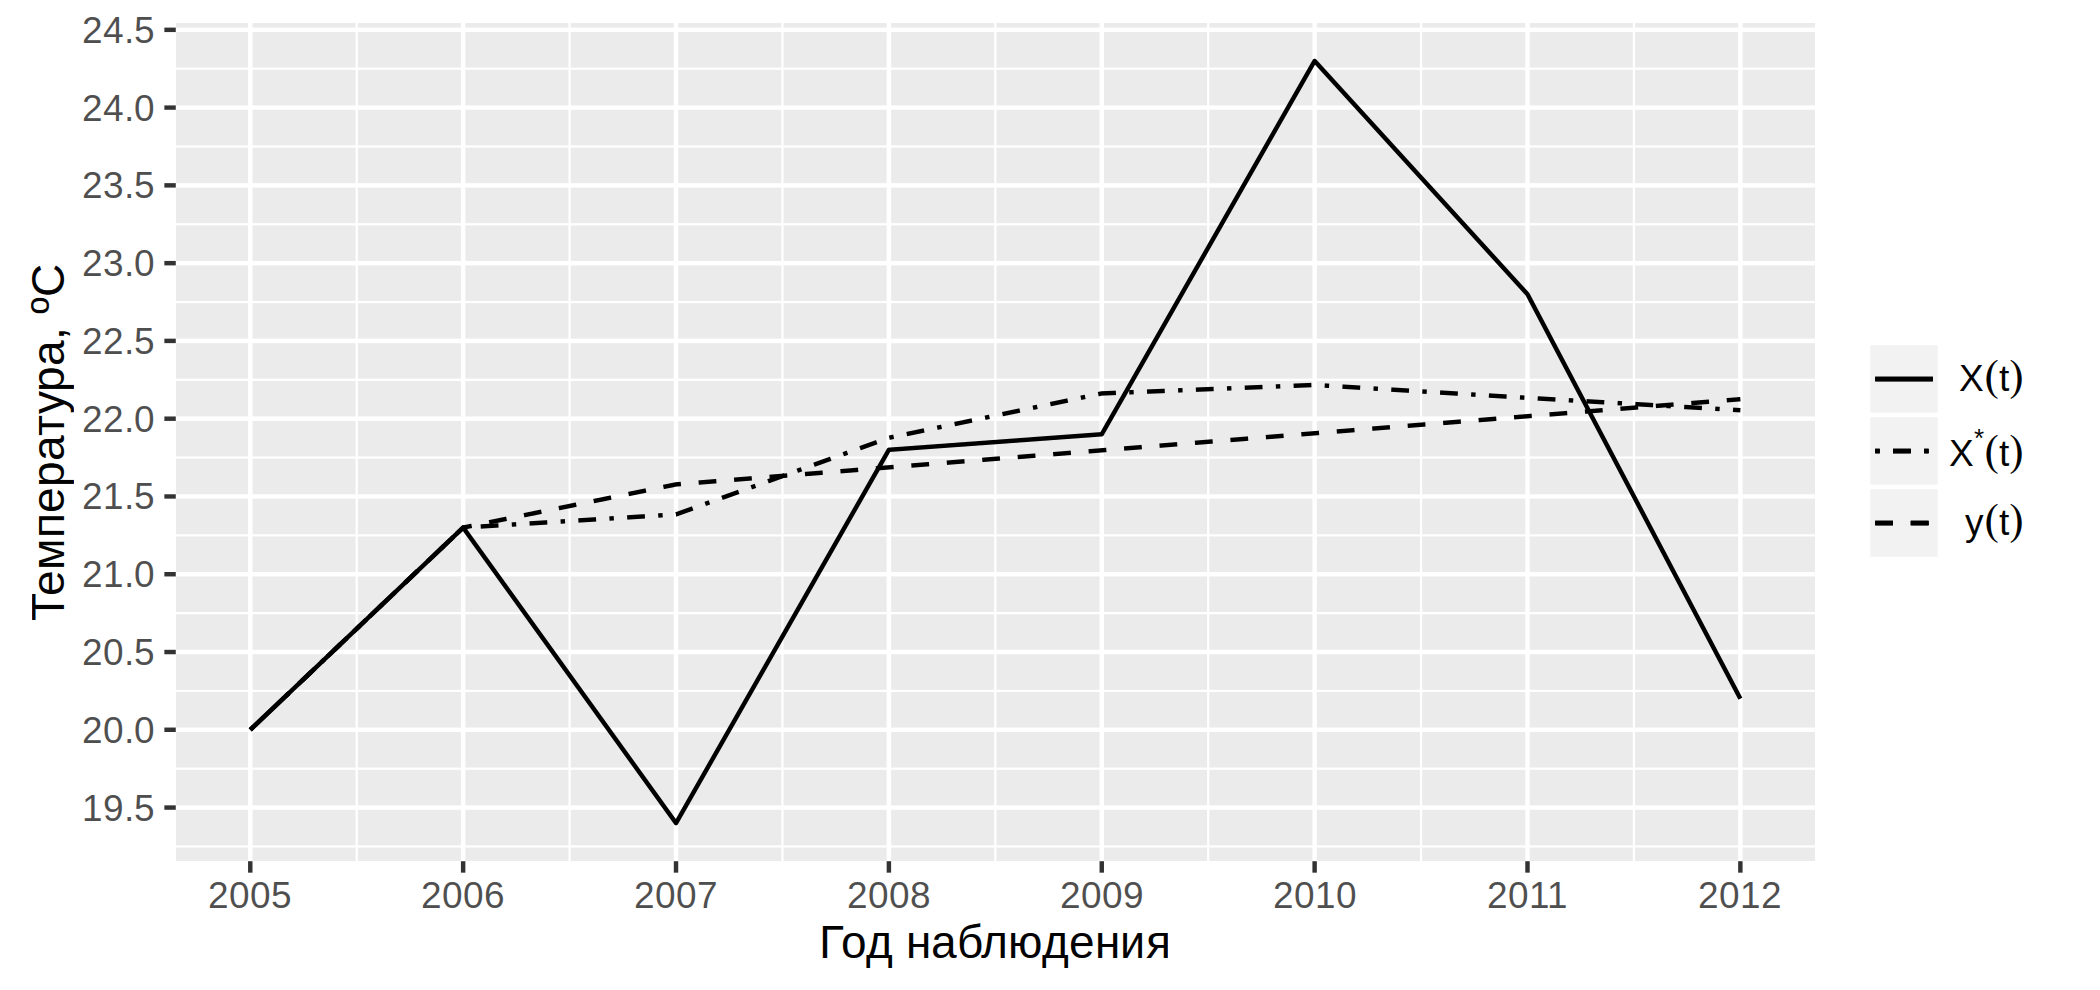
\includegraphics[width=0.9\linewidth]{../../figures/variogram/auto-rob-5-cross-prediction.png}
    \caption{Прогноз по модели $\widehat{\gamma}_6(h)$}
  \end{figure}
  \end{columns}
\end{frame}

\begin{frame}
  \frametitle{Первые два момента оценки вариограммы}
\begin{Theorem}
\begin{footnotesize}
  Для оценки $ 2 \tilde{\gamma}(h) $ имеют место следующие соотношения:
\end{footnotesize}
  \begin{equation*}
    E \{2 \tilde{\gamma}(h) \} = 2 \gamma(h), % DIRTY HACK
  \end{equation*}
  \begin{eqnarray*}
    cov(2 \tilde{\gamma}(h_1), 2 \tilde{\gamma}(h_2)) = \frac{2}{(n - h_1)(n - h_2)} \sum_{t = 1}^{n - h_1}\sum_{s = 1}^{n - h_2} (\gamma(t - h_2 - s) + \\
    + \gamma(t + h_1 - s) - \gamma(t - s) - \gamma(t + h_1 - s - h_2))^2,
  \end{eqnarray*}
  \begin{equation*}
    V \{ 2 \tilde{\gamma}(h) \} = \frac{2}{(n-h)^2}\sum_{t,s = 1}^{n - h} ( \gamma(t - h - s) + \gamma(t + h - s) - 2\gamma(t - s) )^2,
  \end{equation*}
\begin{footnotesize}
  где $ \gamma(h), h \in \mathbb{Z} $, --- семивариограмма процесса $ X(t) $, $ ~h,~ h_1,~ h_2 = \overline{0, n - 1} $.
\end{footnotesize}
\end{Theorem}
\end{frame}

\begin{frame}
  \frametitle{Асимптотическое поведение оценки вариограммы}
  \begin{Theorem}
  \begin{footnotesize}
  Если имеет место соотношение $ \sum_{h = -\infty}^{+\infty} \vert \gamma(h) \vert < +\infty $, то
  \end{footnotesize}
  \begin{eqnarray*}
    \lim_{n \to \infty} (n - \min\{ h_1, h_2 \}) cov\{ 2 \tilde{\gamma}(h_1), 2 \tilde{\gamma}(h_2) \} = \nonumber \\
    = 2 \sum_{m = -\infty}^{+\infty} \gamma(m - h_2) + \gamma(m + h_1) - \gamma(m) - \gamma(m + h_1 - h_2))^2,
  \end{eqnarray*}
  \begin{equation*}
    \lim_{n \to \infty} (n - h) V\{ 2 \tilde{\gamma}(h) \} = 2 \sum_{m = -\infty}^{+\infty} \gamma(m - h) + \gamma(m + h) - 2 \gamma(m))^2,
  \end{equation*}
  \begin{footnotesize}
  где $ \gamma(h), h \in \mathbb{Z} $, --- семивариограмма процесса $ X(t) $, $ h, h_1, h_2 = \overline{0, n - 1} $.
  \end{footnotesize}
\end{Theorem}
\end{frame}

\begin{frame}
  \frametitle{Асимптотическое поведение оценки вариограммы}
  \begin{Corollary}
    Из теоремы 2 вытекает соотношение
    \begin{equation*}
      \lim_{n \to \infty} V\{ 2 \tilde{\gamma}(h) \} = 0, \quad h = \overline{0, n - 1}
    \end{equation*}
  \end{Corollary}

  \begin{Corollary}
    В силу показанной в теореме 1 несмещённости оценки и вышеприведённого следствия получаем, что оценка вариограммы $ 2\tilde{\gamma}(h) $ является состоятельной в среднеквадратическом смысле для вариограммы $ 2\gamma(h), h \in \mathbb{Z} $.
  \end{Corollary}
\end{frame}

\begin{frame}
  \frametitle{Заключение}
  \setlength{\itemindent}{-.5in}
  \begin{columns}
  \column{1.1\linewidth}
  \vspace{-9pt}
  \begin{enumerate}
    \item Проведён предварительный статистический анализ данных:
      \begin{itemize}
        \item показана близость выборочного распределения к нормальному \normaldistr ;
        \item выявлена умеренная положительная зависимость температуры от времени;
        \item построена линейная регрессионная модель;
        \item вычислен и исследован ряд остатков;
      \end{itemize}
    \item Выполнен вариограммный анализ:
      \begin{itemize}
        \item Рассмотрены два подхода по подбору моделей семивариограмм: \small{визуальный и автоматический};
        \item Визуальным подходом показано, что линейная модель с порогом \eqref{eq:gamma4} и периодическая \eqref{eq:gamma6} являются наилучшими;
        \item Автоматическим подходом показано, что волновая \eqref{eq:gamma9} и периодическая \eqref{eq:gamma10} являются наилучшими;
      \end{itemize}
  \end{enumerate}
  \end{columns}
\end{frame}

\begin{frame}
  \frametitle{Заключение}
  \setlength{\itemindent}{-.5in}
  \begin{columns}
  \column{1.1\linewidth}
  \vspace{-9pt}
  \begin{enumerate}
    \item[3.] По различным моделям построены прогнозные значения методом кригинг. Исследована зависимость точности прогноза от оценки вариограммы и модели;
    \item[4.] Исследованы статистические свойства оценки вариограммы гауссовского случайного процесса. Показана несмещённость и состоятельность в среднеквадратическом смысле оценки вариограммы \eqref{eq:matheron};
    \item[5.] Реализовано программное обеспечение для решения класса задач, аналогичных исходной.
  \end{enumerate}
  \end{columns}
\end{frame}

\begin{frame}
  \frametitle{Список использованных источников}
  \begin{scriptsize}
  \begin{thebibliography}{5}
    \beamertemplatebookbibitems
    \bibitem{cressie}
      Cressie~N.
      \newblock {\em Statistics for Spatial Data}.
      \newblock New York. --- Wiley, 1993.
    \beamertemplatebookbibitems
    \bibitem{saveliev}
      А.А.~Савельев, С.С.~Мухарамова, А.Г.~Пилюгин, Н.А.~Чижикова
      \newblock {\em Геостатистический анализ данных в экологии и природопользовании (с применением пакета R)}
      \newblock Казань: Казанский университет, 2012.
    \beamertemplatebookbibitems
    \bibitem{true}
      Н.Н.~Труш
      \newblock {\em Асимптотические методы статистического анализа временных рядов.}
      \newblock Белгосуниверситет, 1999.
    \beamertemplatebookbibitems
    \bibitem{shumway}
      Robert H.~Shumway, David S.~Stoffer
      \newblock {\em Time series and Its Applications: With R Examples (Springer Texts in Statistics)}.
      \newblock Springer Science+Business Media, LLC 2011, 3d edition, 2011.
    \beamertemplatebookbibitems
    \bibitem{cook}
      Paul~Teetor
      \newblock {\em R Cookbook (O’Reilly Cookbooks)}.
      \newblock O’Reilly Media, 1 edition, 2011.
    \beamertemplatearticlebibitems
    \bibitem{mingoti}
      Mingoti~Sueli~Aparecida, Rosa~Gilmar
      \newblock A note on robust and non-robust variogram estimators
      \newblock {\em Rem: Revista Escola de Minas.}, Vol. 61:87–95, 2008.
  \end{thebibliography}
\end{scriptsize}
\end{frame}

\begin{frame}
  \frametitle{\null}
  \begin{center}
    {\Huge Спасибо за внимание!}
  \end{center}
\end{frame}

\end{document}